%%%%%%%%%%%%%%%%%%%%%%%%%%%%%%%%%%%%%%%%%%%%%%%%%%%%%%%%%%%%%%%%%%%%%%%%%%%%%%%
%Objetivo: Mapeamento Sistemático da Literatura com o objetivo de avaliar
%		   o que está sendo proposto de melhorias nas funcionalidades das
% 		   FGRM
%Autor: Vagner Clementino e Rodolfo Resende
%Criação: Ter Out 11 19:03:45 BRT 2016
%Modificação: seg dez 19 21:41:29 BRST 2016
%Revisão:
%%%%%%%%%%%%%%%%%%%%%%%%%%%%%%%%%%%%%%%%%%%%%%%%%%%%%%%%%%%%%%%%%%%%%%%%%%%%%%%

\chapter{Mapeamento Sistemático da Literatura}
\label{ch:mapeamento-sistematico}

\section{Introdução}
\label{sec:map-intro}
\todo[inline]{OBJETIVO DA SEÇÃO\@: Esta seção visa apresenta uma visão geral do
	Mapeamento Sistemático realizado. Apresenta, de maneira sucinta, o contexto,
	o problema, a solução e os resultado deste estudo, de forma resumida, mas
	abrangente. Idealmente deverá ser a última seção a ser escrita neste
	Capítulo.}

\section{Metodologia de Pesquisa}
\label{sec:map-metodologia}

Um \textit{Mapeamento Sistemático da Literatura}, também conhecido como Estudo
de Escopo (Scoping Studies), tem como seus objetivos fornecer uma visão geral de
determinada área de pesquisa, estabelecer a existência de evidências de estudos
sobre determinado tema e fornecer uma indicação da quantidade de trabalho da
linha de pesquisa sob
análise~\cite{keele2007guidelines,wohlin2012experimentation}. Nesta dissertação
empregamos as diretrizes propostas por Petersen e outros~\cite{Petersen2008} de
forma a produzirmos uma revisão de maneira sistemática afim de propiciar maior
facilidade de replicação e extensão do mapeamento realizado. Em particular,
definimos um conjunto de questões de pesquisa que foram utilizadas no processo
de busca e seleção dos estudos primários. Em seguida, foram construídos esquemas
de classificação com base nos dados extraídos dos artigos. Por fim, foi
realizada a análise e sintetização dos dados com o objetivo de posicionar os
estudos em suas respectivas classes na taxonomia. A estrutura desta seção está
de acordo com o processo descrito por \textit{Petersen e outros}, de modo que
cada subseção representa uma das etapas propostas pelos autores.

\subsection{Questões de Pesquisa}
\label{subsec:map-questoes-de-pesquisa}

O objetivo deste mapeamento sistemático é entender o estado da arte da pesquisa
sobre FGRM\@. Em especial, o foco é identificar as extensões que estão sendo
propostas para este tipo de ferramenta.  No escopo deste trabalho, uma extensão
é um componente de software que adiciona uma característica específica para um
programa de
computador\footnote{\url{https://en.wikipedia.org/wiki/Plug-in_(computing)}}.
Assim, a fim de alcançar e guiar os objetivos desta parte do trabalho, foram
definidas as seguintes questões de pesquisa:

\todo[inline]{Incluir motivação das questões de pesquisa}

\begin{itemize}
	\item \textbf{Questão 01}: \textit{Quais os problemas da atividade de
			manutenção de software as extensões das FGRM pretendem resolver?}
	\item \textbf{Questão 02}: \textit{Quais papeis envolvidos no processo de
			manutenção de software as extensões visam dar suporte?}
	\item \textbf{Questão 03}: \textit{Qual o modelo de Recuperação da
			Informação foi utilizada para desenvolver a extensão?}
	\item \textbf{Questão 04}: \textit{Quais as FGRM disponíveis no mercados
			estão sendo estendidas?}

\end{itemize}

\subsection{Pesquisa da Literatura}
\label{subsec:map-pesquisa-literatura}

Com o objetivo de encontrar o conjunto de estudos mais relevantes, bem como
eliminar aqueles que não são capazes de responder as questões de pesquisas
propostas, adotamos os seguintes critérios para inclusão ou exclusão dos
estudos:

\begin{itemize}
	\item Critérios de Inclusão
		\begin{itemize}
			 \item Artigos publicados em conferências e periódicos (journals)
			 \item Estudos publicados a partir de 2010\footnote{Foram
					 considerados neste estudo artigos publicados até maio/2016,
					 data de realização da pesquisa nas base de dados.}
			 \item Artigos escritos em língua inglesa e portuguesa
			 \item Artigos disponíveis com texto completo
		\end{itemize}
	\item Critérios de Exclusão
		\begin{itemize}
			\item Livros e literatura cinza (gray literature)
			\item Artigos que não possuem relação com FGRM
			\item Estudos duplicados, neste caso apenas foi considerada a versão
				mais completa do trabalho
		\end{itemize}
\end{itemize}

Os estudos primários foram coletados mediante a aplicação de sentenças de buscas
nas seguintes bibliotecas digitais: \textit{IEEE Explore, ACM Digital Library,
	Scopus, e Inspec/Compendex}. As bases de dados foram escolhidas com base na
experiência reportada por Dyba e outros~\cite{dybaa2007applying}  no qual
verificou-se que o uso de apenas algumas bases era capaz de produzir um
resultado similar a utilização de um conjunto maior de biblioteca digitais. As
sentenças de buscas foram produzidas com base na metodologia PICO (Population,
Intervention, Comparison and Outcomes) que é sugerida por Kitchenham e
Charters~\cite{keele2007guidelines} para ajudar pesquisadores na formulação de
termos tomando como base as questões de pesquisa, que serão aplicados às bases
de dados. As sentenças de busca aplicadas a cada base de dados são apresentadas
na Tabela~\ref{tab:setenca-por-base-dados} do
Apêndice~\ref{ch:app-instrumentos-mapeamento}.

Após a condução da busca automatizada nas base de dados chegamos a um total de
286 artigos. A Tabela~\ref{tab:estudos-por-base-dados} exibe o conjunto inicial
de estudos recuperados por base de dados.  Os trabalhos coletados foram
avaliados, através da ferramenta
\textit{JabRef}\footnote{\url{https://www.jabref.org/}}, em busca de possíveis
duplicados tendo em vista a utilização de diferentes bases de dados. A busca por
artigos duplicados resultou na exclusão de 81 documentos de modo que obtivemos
um total de 205 estudos ao final do processo. Finalmente os artigos foram
analisados com base na leitura do título e resumo. Nos casos em que o título e
resumo não eram capazes de caracterizar o estudo uma leitura completa do texto
foi realizada. O processo descrito resultou em 94 estudos incluídos neste
trabalho. A Figura~\ref{fig:diagrama-processo-selecao}

\todo[inline]{Verificar o processo com objetivo de validar o total de artigo em
	cada etapa do processo.}

\begin{figure}
	\centering
	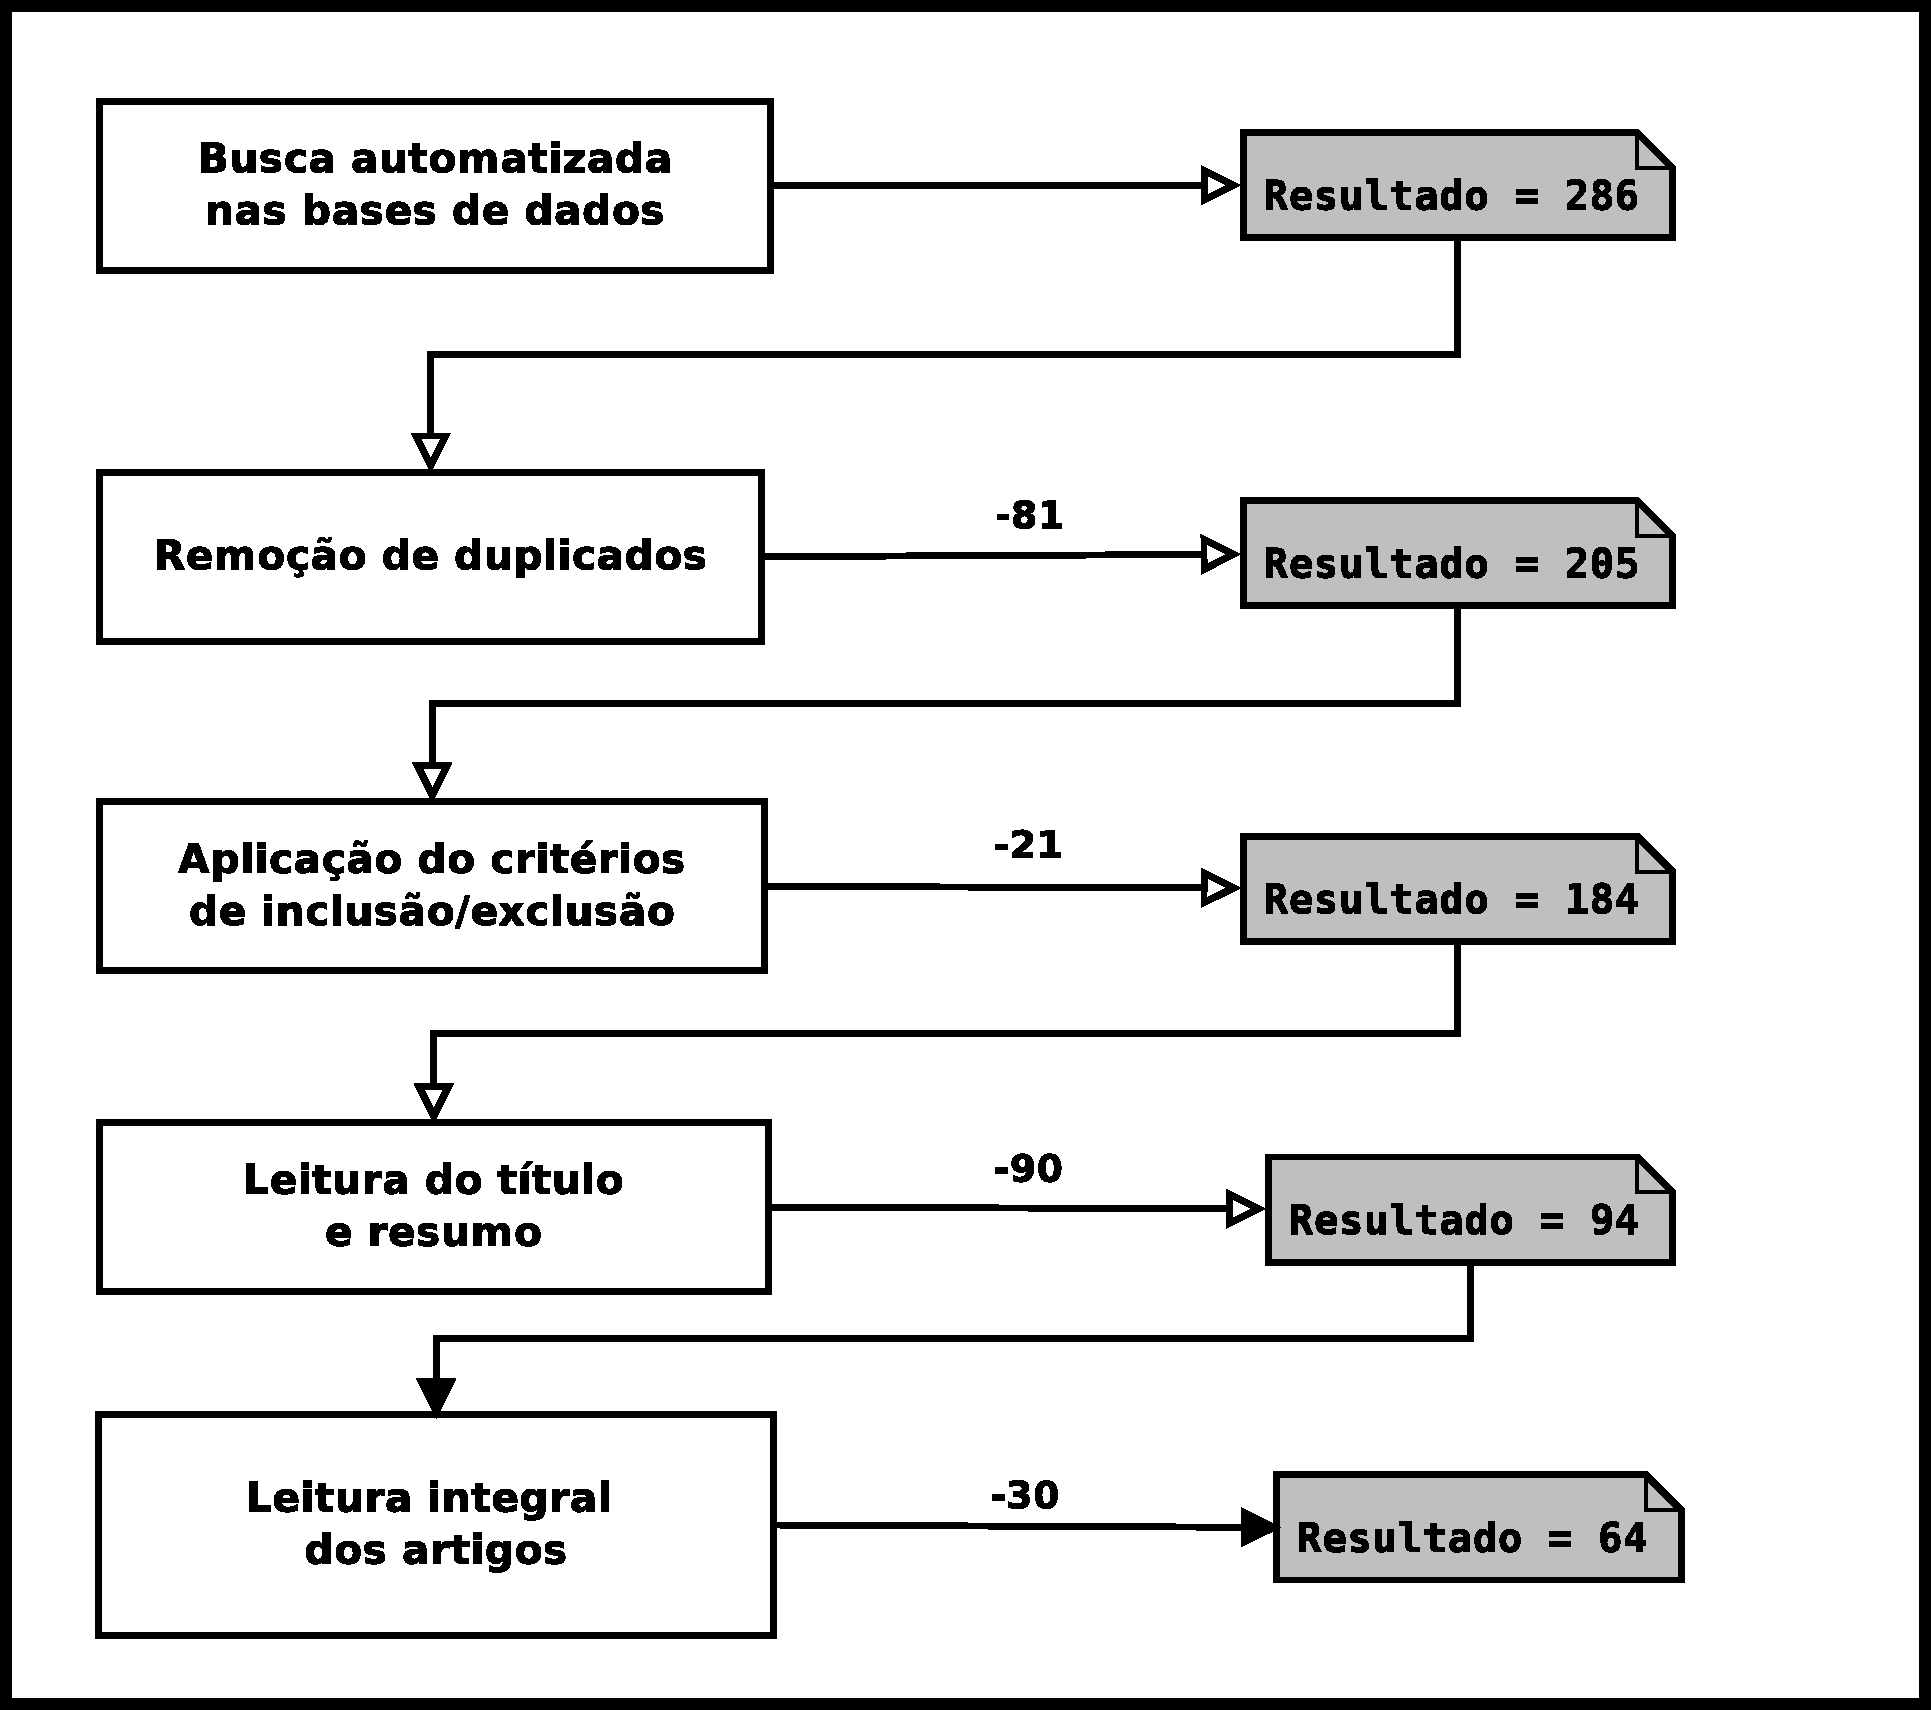
\includegraphics[width=0.75\linewidth]
	{./chapter-mapeamento-sistematico/img/diagrama-processo-selecao.pdf}
	\caption{Número de artigos incluídos durante o processo de seleção dos
		estudos. Baseado
		em~\cite{Petersen2015}}\label{fig:diagrama-processo-selecao}
\end{figure}

\begin{table}[htb]
	\centering
	\caption{Número de Estudos Recuperados por Base de Dados}\label{tab:estudos-por-base-dados}
	\begin{tabular}{cc}
		\hline
		\textbf{Base de Dados} & \textbf{Total} \\ \hline
		ACM Digital Library    & 109            \\
		IEEE Explore           & 100            \\
		Inspec/Compendex       & 22             \\
		Scopus                 & 55             \\ \hline
	\end{tabular}

\end{table}

\subsection{Esquemas de Classificação}
\label{subsec:map-esquemas-classificacao}

Com o objetivo de mapear os estudos sobre extensões das FGRM's foram propostos
quatro esquemas de classificação. O primeiro esquema organiza os artigos pelo
tipo de problema da atividade de manutenção de software a extensão se propõe
solucionar. A segunda categorização distribuí os estudos pelo papel no processo
de manutenção de software a extensão visa dar suporte. A terceira é uma
classificação baseada na taxonomia para modelos de Recuperação da Informação
(Information Retrieve~-~IR) proposta por Cerulo e
Canfora~\cite{cerulo2004taxonomy}. Em particular, utilizamos este esquema tendo
em vista que grande parte das extensões propostas na literatura utilizam algum
tipo de suporte de modelos de IR\@. O último esquema apresenta quais das
ferramentas existentes na indústria estão sendo estendidas na literatura. Esta
taxonomia nos fornece uma visão se as extensões propostas são com um foco
propositivo, ou seja, sem que exista uma implementação concreta da extensão, ou
se há algum tipo de ferramenta no qual existe um maior número de extensões
propostas. Em seguida discutiremos cada esquema de classificação em detalhe.

\subsubsection{Classificação por Tipo de Problema}
\label{subsubsec:map-esquema-suporte-problema}

Existem diversos problemas relacionados ao processo de Manutenção de Software.
Já na década de 1980 pesquisas questionavam os profissionais envolvidos com
manutenção de software quais os principais problemas da
área\cite{Lientz:1981:PAS:358790.358796}. Naturalmente a percepção dos desafios
envolvidos com a manutenção de software se altera com tempo, desta forma, é
sempre válido revisar a literatura com o objetivo de entender quais os tipos de
problemas estão sendo estudados.

Neste sentido foi proposto um esquema de classificação que relaciona os estudos
pelo tipo de problema que a extensão pretende resolver. A construção da
taxonomia se deu com base no processo definido por Petersen e
outros~\cite{Petersen2008}, o qual é composto de duas etapas:

\begin{enumerate}[I]
	\item analisar as palavras-chaves e conceitos que identificam as
		contribuições do estudo por meio da analise do título e resumo
	\item após o término da etapa I, todas as palavras chaves são combinadas a
		fim de construir um conjunto de categorias para no qual os artigos devem
		ser classificados.
\end{enumerate}

Os autores recomendam que nos casos em que o resumo e o título do estudo não
sejam capazes de caracterizá-lo, as seções de introdução e conclusão também
devem ser analisadas. Para as bases de dados onde era informado mais de um
conjunto de palavras-chaves para um mesmo artigo, utilizamos aquelas que foram
informadas pelos autores. Mediante a aplicação do processo foi construído o
esquema de classificação apresentado na
Figura~\ref{fig:diagrama-esquema-dimensao-melhorias}.

\begin{figure}[tb]
\centering
 \makebox[\textwidth]{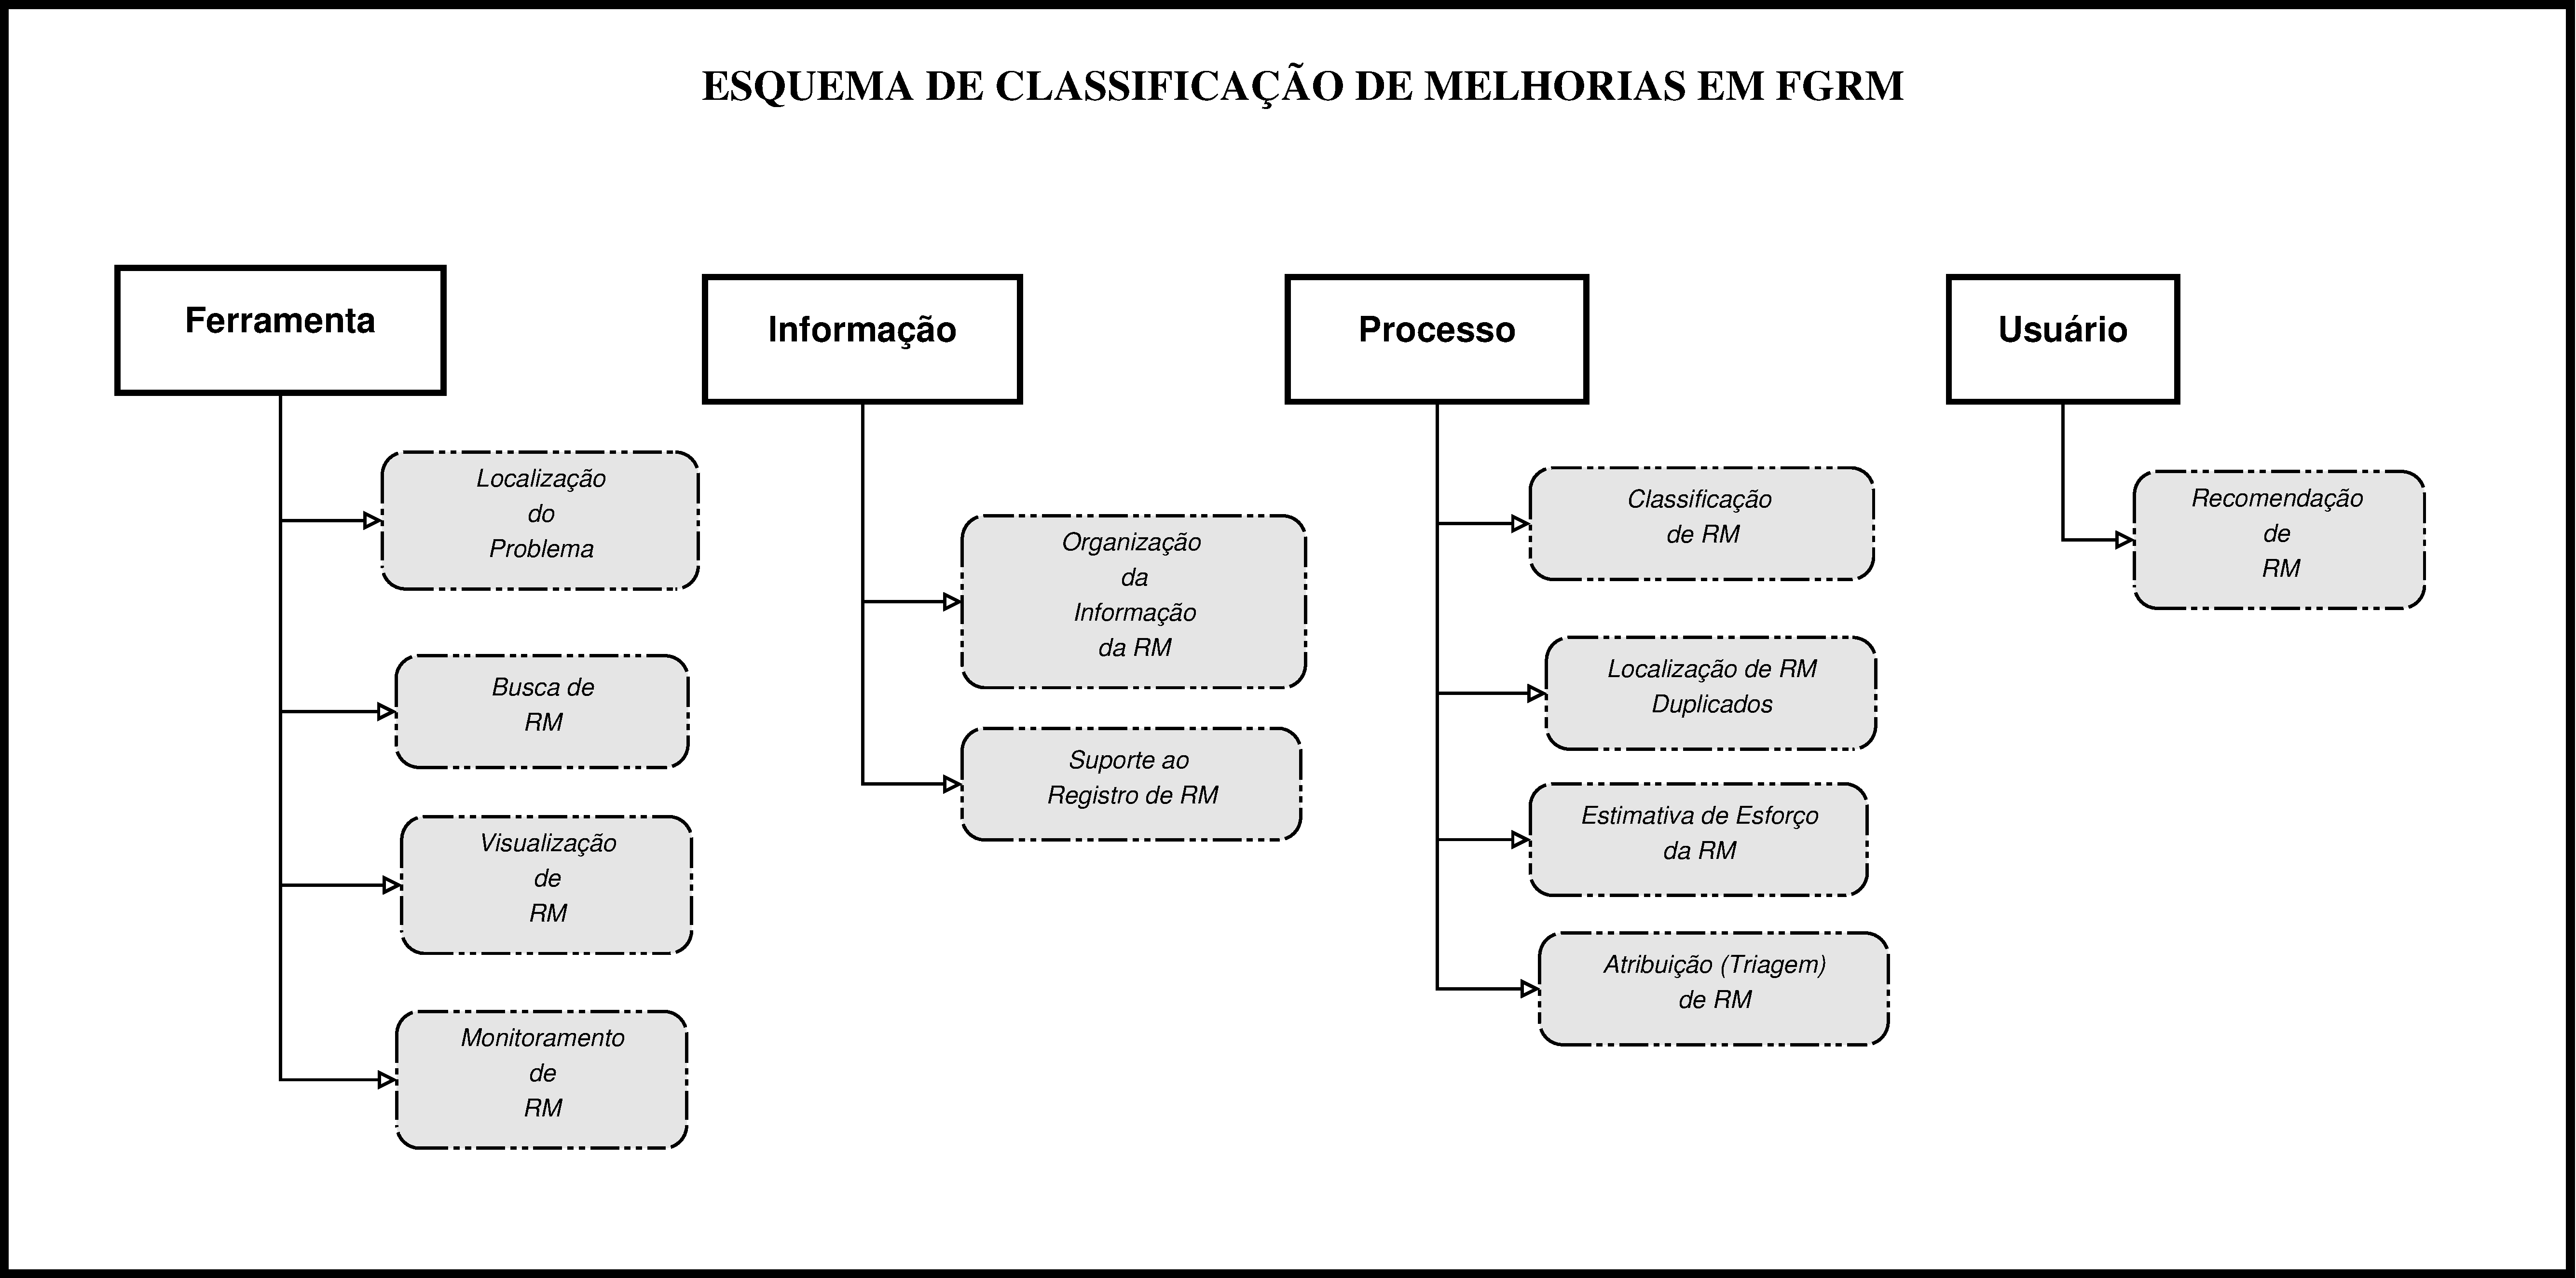
\includegraphics[width=.9\paperwidth]{./chapter-mapeamento-sistematico/img/diagrama-esquema-dimensoes-melhorias.pdf}}
\caption{Esquema de classificação das melhorias propostas na literatura. Os
	retângulos representam as dimensões de melhorias e os polígonos de cantos
	arredondados representam as melhorias.}
\label{fig:diagrama-esquema-dimensao-melhorias}
\end{figure}
\todo[inline]{Incluir no anexo uma tabela demonstrando como as palavras-chaves foram combinadas}


\subsubsection{Classificação por Suporte ao Papel da Manutenção de Software}
\label{subsubsec:map-esquema-suporte-papel-man}

Da mesma forma que uma extensão proposta para as FGRM's visa resolver
determinado problema, supomos ainda que a extensão pode dar suporte a
determinado papel desempenhado no processo de Manutenção de Software. Para este
fim utilizamos uma classificação modificada da proposta por~\cite{Polo1999}. No
trabalho de Polo e outros o objetivo era definição de uma estrutura adequada da
equipe de manutenção de software mediante a clara identificação das tarefas que
cada membro deve executar. Os papéis propostos pelo no estudo é produto da
aplicação da metodologia MANTEMA~\cite{756695} para manutenção em projetos de
software bancários espanhóis, em especial aqueles em que a área de manutenção
foi terceirizada (outsourcing). Os autores reforçam que apesar da taxonomia de
papéis ter sido criada em um contexto específico, ela pode ser adequada para
aplicação em outras situações.

No escopo deste trabalho a taxonomia utiliza a proposta de Polo e outros com
algumas adequações. Em especial, foram removidos os papéis que segundo o nosso
entendimento estão mais vinculados a um contexto de manutenção terceirizada
(outsourcing). Além disso, dividimos o papel ``time de manutenção' (maintenance
team) em \textit{Desenvolvedor e Analista de Qualidade} por entendemos que são
papéis comuns a muito dos processos de manutenção existentes. Os papéis que
compõe a taxonomia proposta estão descritos a seguir:

\begin{description}
	\item[Usuário Afetado]: Indivíduo que utiliza o sistema do qual será
		produzida uma Requisição de Mudança.
	\item[Reportador]: Responsável por registrar a Requisição de Mudança na
		FGRM\@.
	\item[Gerente de Requisição de Mudança (Maintenance-request manager)]:
		Responsável por decidir se uma Requisição de Mudança será aceita ou
		rejeitada e qual tipo de manutenção deverá ser aplicada. Posteriormente
		cabe a ele/ela encaminhar a RM para o Agendador.
	\item[Agendador (Scheduler)]: Deve planejar a fila de Requisições de Mudança
		aceitas. Também estão no rol de responsabilidades deste papel a
		atribuição das RM's para o desenvolver mais apto.
	\item[Desenvolvedor]: Responsável realizar as ações que irão solucionar a
		Requisição de Mudança.
	\item[Analista de Qualidade]: Avaliam uma Requisição de Mudança que foi
		solucionada por um Desenvolvedor afim de verificar se a RM foi
		corretamente resolvida.
	\item[Líder da Manutenção (Head of Maintenance)]: Tem por responsabilidade
		definir os padrões e procedimentos que compõe o processo de manutenção
		que será utilizado.
\end{description}

Apesar da taxonomia de papéis utilizada derivar de um contexto de manutenção de
software específico (setor bancário e empresas com a área de manutenção
terceirizada), ela é capaz de acoplar com outros tipos de processo de manutenção
de software, como aquele proposto por Ihara e outros
\cite{Ihara:2009:AMI:1595808.1595833}. Naquele estudo foi criada uma
representação de um processo de modificação de bugs tomando como base as
diversas situações que um bug possui em uma FGRM no contexto de projetos de
código aberto. O processo resultante é facilmente acoplável com a taxonomia
utilizada em nosso estudo.

Cabe ressaltar que está fora do escopo deste estudo elaborar uma taxonomia de
papeis envolvidos na Manutenção de Software em função de supormos que isto
corresponde a um esforço bem extenso. Nossa ação é identificar quais artigos
trabalham com a noção de quais papeis a extensão pretender dar suporte,  ou
seja,  relatar se existem papeis e quais são eles,  sem com isso, envolver em
uma consolidação definitiva.

\subsubsection{Classificação por Técnicas de Recuperação da Informação}
\label{subsubsec:map-esaquema-tecnicas-ir}

Um ponto em comum entre as diversas extensões para FGRM propostas na literatura
é o fato delas utilizarem algum suporte de modelos de Recuperação de Informação
(Information Retrieve~-~IR). Um modelo de IR visa solucionar um uma necessidade
informacional de um usuário, representada como um conjunto de termos, no qual
uma lista dos documentos mais relevantes devem ser recuperadas de uma
coleção~\cite{baeza1999modern}.

Com o objetivo de obter uma visão geral das técnicas que estão sendo utilizadas
para implementar as extensões para as FGRM, realizamos a classificação dos
estudos através da taxonomia proposta por Canfora e
Cerulo\cite{cerulo2004taxonomy}. O esquema de classificação consiste em duas
visões sobrepostas: uma taxonomia vertical que classifica os modelos de IR com
relação ao seu conjunto de características básicas; e uma taxonomia horizontal
que classifica os objetos de IR com respeito as suas tarefas, forma e
contexto\cite{cerulo2004taxonomy}. Nesta dissertação utilizamos a classificação
vertical tendo em vista que estamos interessados na técnica utilizada na
implementação da extensão.

\todo[inline]{Verificar a necessidade de definir melhor alguns termos de IR\@.
	Ex\@. documento, consulta do usuário, problema da representação de
	similaridade}

\todo[inline]{Verificar o total de artigos que utilizam algum técnica de IR\@.
	Apesar de grande parte utilizar não serão todos os artigos}

A taxonomia vertical é construída explorando duas características básicas de um
Modelo de Recuperação da Informação: \textit{representação (representation)},
que é a forma adotada para representar ao mesmo tempo o documento e consulta do
usuário; \textit{raciocínio (reasoning)}, ao qual se refere ao framework adotado
para resolver o problema da representação de similaridade, ou seja, trata-se do
conjunto de métodos, modelos e tecnologias utilizadas para realizar o casamento
entre um documento e a consulta do usuário. O esquema de classificação proposto
pelos autores é apresentado na Figura~\ref{fig:information-retrieval-model}.

\begin{figure}[htpb]
	\centering
	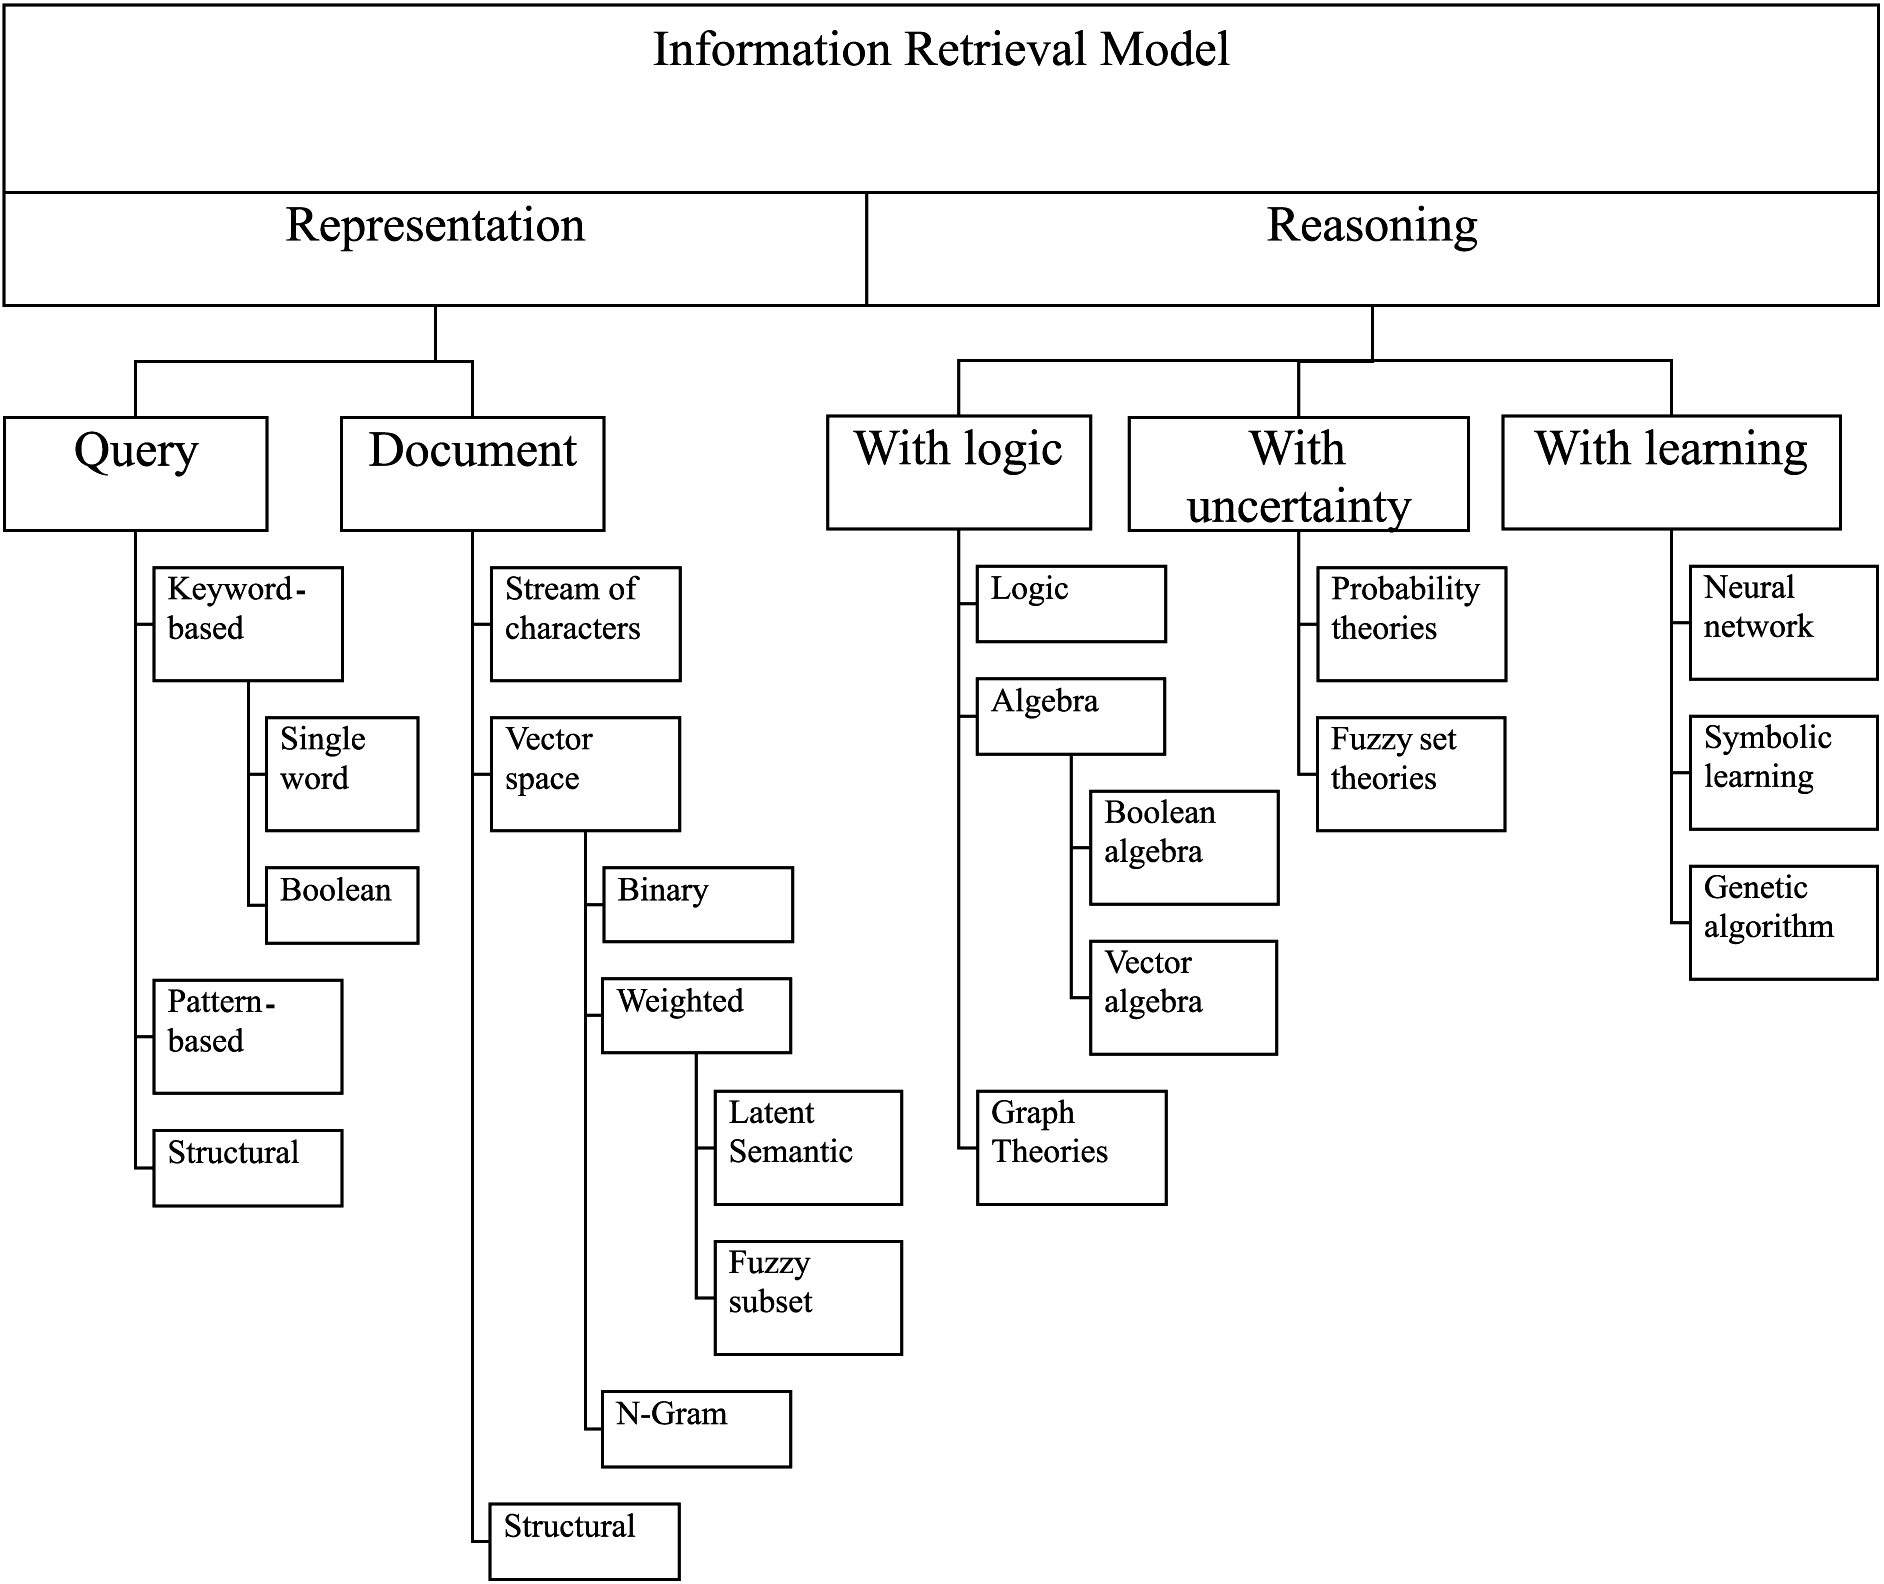
\includegraphics[width=0.8\linewidth]{./chapter-mapeamento-sistematico/img/information-retrieval-model.png}
	\caption{Taxonomia vertical para Modelos de Recuperação da Informação.
		Adaptado
		de~\cite{cerulo2004taxonomy}}\label{fig:information-retrieval-model}
\end{figure}

\subsubsection{Classificação por Ferramenta Estendida}
\label{subsubsec:map-esquema-ferramenta}

Do ponto de vista dos profissionais envolvidos em Manutenção de Software é
importante entender quais as FGRM estão sendo estendidas. Por outro lado, para
os pesquisadores é importante descobrir aquelas ferramentas mais ``amigáveis
para o desenvolvimento de novas extensões bem como a melhoria das existentes.
Neste sentido, realizamos a classificação dos estudos pelas ferramentas que
foram utilizados para o desenvolvimento das extensões. Uma ferramenta é
entendida como utilizada por determinado estudo se ela foi utilizada no processo
de validação ou se seus dados foram utilizados na avaliação da extensão.

Para produzirmos a taxonomia realizarmos a leitura do resumo e da introdução do
artigo. Nos casos em que não foi possível determinar a ferramenta utilizada a
partir da leitura das seções citadas, procedemos com a leitura com a parte
avaliação do estudo. A Tabela exibe as ferramentas utilizadas para cada estudo
analisado.

\section{Resultados}
\label{sec:resultados}

Nesta seção apresentamos os resultados do Mapeamento Sistemático. Cada uma das
taxonomias propostas é analisada mediante a apresentação dos estudos que possam
exemplificar a classificação adotada.  Iniciamos com uma análise da frequência
de publicação relativo à melhoria das funcionalidades das ferramentas.
Posteriormente apresentamos os resultados pela classificação por problemas na
Manutenção de Software, o qual dividimos os estudos por área e tópico de
pesquisa. Seguimos com a análise dos estudo pelo papel ao qual a extensão visa
dar suporte. Posteriormente analisamos os modelos de IR utilizados para
implementar algumas das extensões propostas na literatura. Finalizamos esta
análise com as ferramentas existentes no mercado que estão efetivamente sendo
entendidas.

\subsection{Frequência das Publicações}
\label{sub:frequencia_publicacao}

A Figura~\ref{fig:publicacao_por_ano} exibe o número de estudos primários
identificados entre os anos 2010@-@2016, período de referência utilizado no
mapeamento. Dentre os estudos escolhidos no período em questão verificamos que
em 2010 foram publicados cinco estudos sobre o assunto
\cite{sun2010discriminative,gegick2010identifying,song2010jdf,nagwani2010predictive,zimmermann2010makes}.
Posteriormente verificamos um acréscimo no número de estudos no qual um
significante aumento pode ser observado entre os anos de 2012@-@2014. O crescente
número de estudos publicados sobre melhorias nas FGRM pode indicar que esta área
vem sendo considerada altamente relevante pela comunidade acadêmica em
Engenharia de Software.

\begin{figure}[htpb]
	\centering
	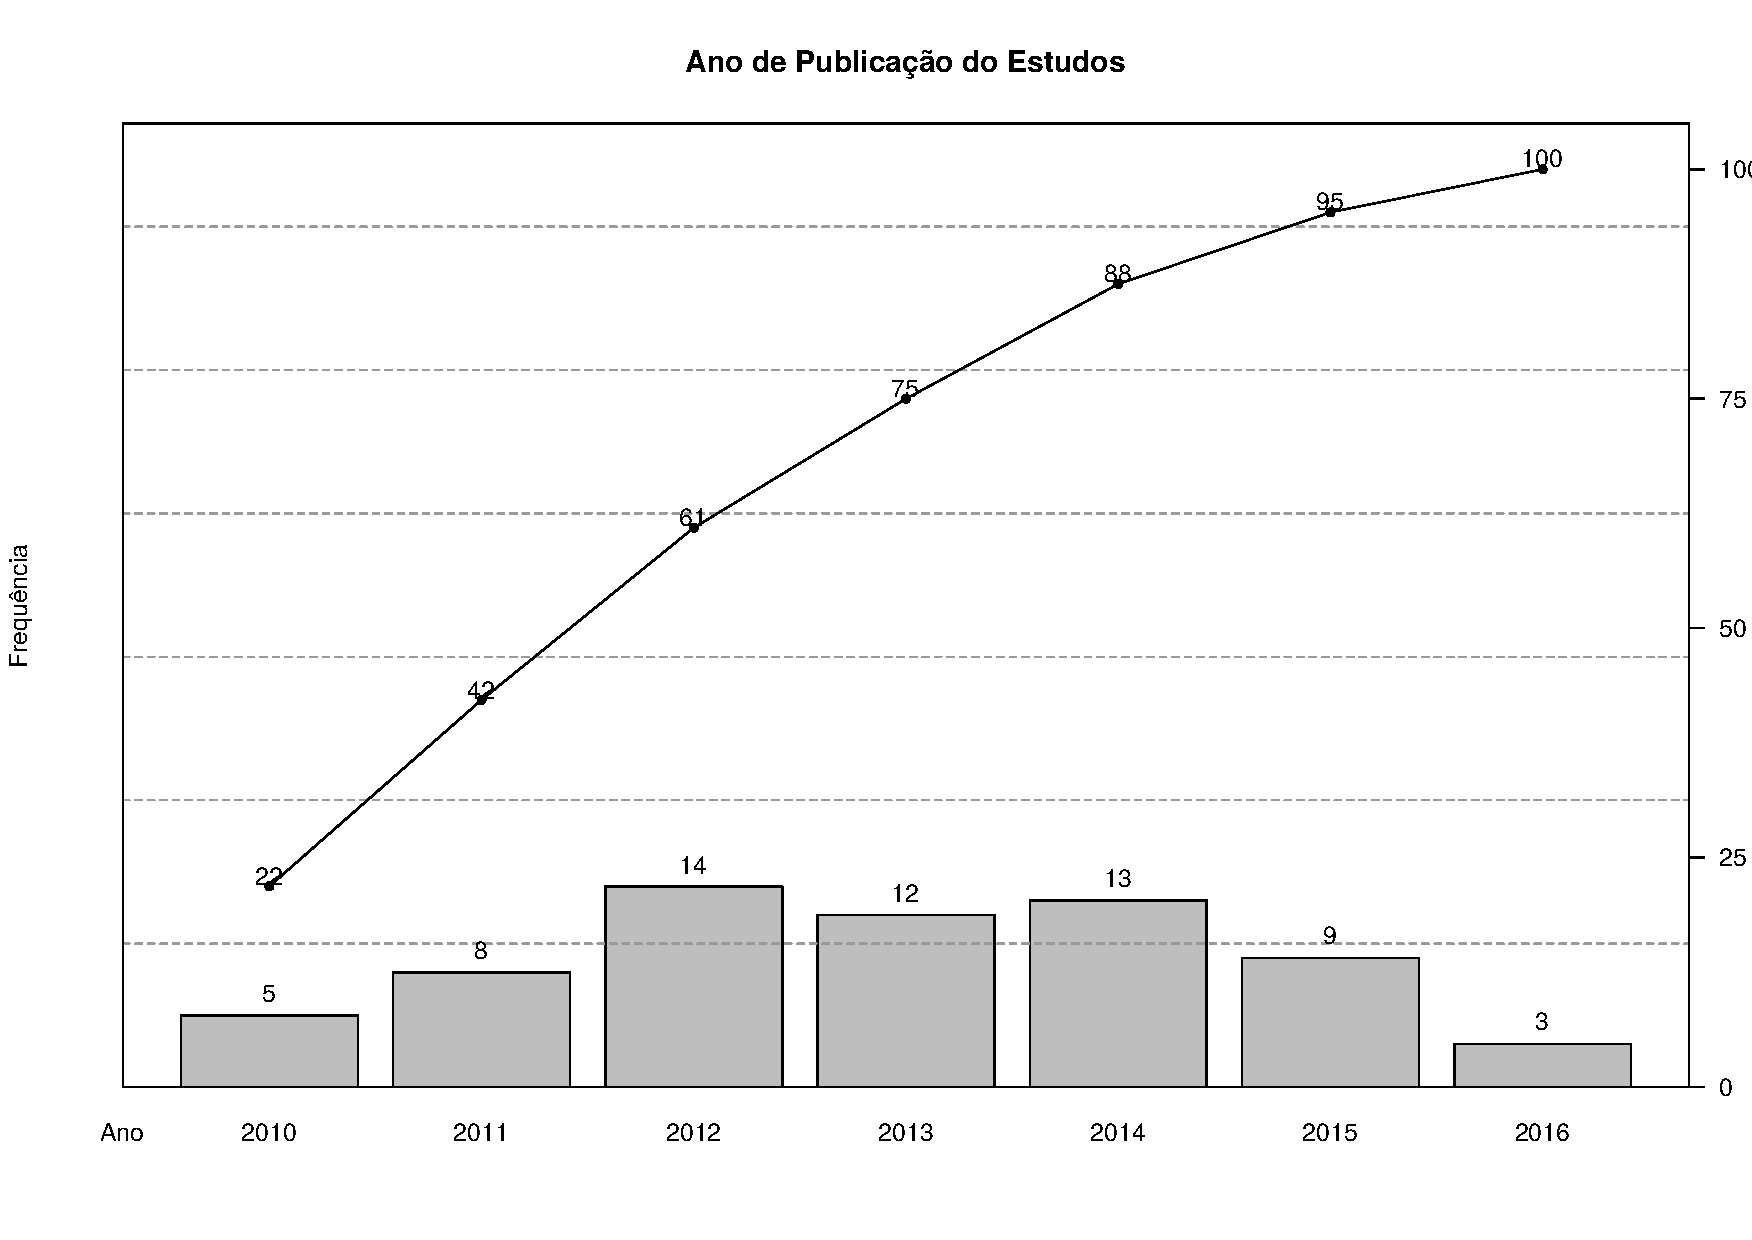
\includegraphics[width=0.9\linewidth]{chapter-mapeamento-sistematico/img/ano-publicao-estudos.pdf}
	\caption{Número de estudos primários por ano de publicação.}
\label{fig:publicacao_por_ano}
\end{figure}

\subsection{Extensões para Problemas na Manutenção de Software}
\label{sub:extensões_para_problemas_na_manutenção_de_software}

Nesta etapa do trabalho estamos interessados no estado da arte do estudo dos
problemas encontrados na Manutenção de Software. Em especial, o nosso foco é
entender que tipo de melhorias nas funcionalidades das FGRM estão sendo proposta
na literatura. Com base no mapeamento sistemático realizado e nas dimensões de
melhoria discutidas por Zimmermann e outros~\cite{5070993} construímos o esquema
de classificação dos apresentado na
Figura~\ref{fig:diagrama-esquema-dimensao-melhorias}

Adicionalmente a tabela~\ref{tab:taxonomia-problemas-manutencao} exibe a
distribuição dos estudos pela dimensão de melhoria e o seu respetivo tópico. De
uma certa maneira o número de estudos  pode indicar a maturidade da pesquisa
naquele tipo de assunto. Contudo, não representa diretamente a importância do
tópico no estudo sobre melhorias em FGRM's.

% Inclusão da tabela
\begin{table}[htbp]
\centering
\caption{My caption}
\label{my-label}
\resizebox{\textwidth}{!}{%
\begin{tabular}{|c|l|l|c|}
\hline
\textbf{Dimensão da Melhoria} & \multicolumn{1}{c|}{\textbf{Tópico}}             & \multicolumn{1}{c|}{\textbf{Estudos}}          & \textbf{Total}       \\ \hline
\multirow{13}{*}{Ferramenta}  & Busca de RM                                      & \cite{Liu2014}                                 & 1                    \\ \cline{2-4} 
                              & \multirow{7}{*}{Localização do Problema}         & \cite{Bangcharoensap:2012:LSC:2419061.2419428} & \multirow{7}{*}{7}   \\
                              &                                                  & \cite{Corley2011}                              &                      \\
                              &                                                  & \cite{Nguyen:2012:MAR:2393596.2393671}         &                      \\
                              &                                                  & \cite{Romo:2015:TAT:2745802.2745833}           &                      \\
                              &                                                  & \cite{thung2013automatic}                      &                      \\
                              &                                                  & \cite{Thung:2014:BIT:2635868.2661678}          &                      \\
                              &                                                  & \cite{Wong:2014:BBF:2705615.2706096}           &                      \\ \cline{2-4} 
                              & Monitoramento de RM                              & \cite{Aggarwal:2014:MIT:2593801.2593810}       & 1                    \\ \cline{2-4} 
                              & \multirow{4}{*}{Visualização de RM}              & \cite{dal2013closer}                           & \multirow{4}{*}{4}   \\
                              &                                                  & \cite{Hora2012}                                &                      \\
                              &                                                  & \cite{Sasso2014}                               &                      \\
                              &                                                  & \cite{takama2013application}                   &                      \\ \hline
\multirow{9}{*}{Informação}   & \multirow{2}{*}{Organização da Informação da RM} & \cite{mani2012ausum}                           & \multirow{2}{*}{2}   \\
                              &                                                  & \cite{Otoom2016}                               &                      \\ \cline{2-4} 
                              & \multirow{7}{*}{Suporte ao Registro da RM}       & \cite{Bettenburg2008a}                         & \multirow{7}{*}{7}   \\
                              &                                                  & \cite{Correa2013b}                             &                      \\
                              &                                                  & \cite{moran2015auto}                           &                      \\
                              &                                                  & \cite{Moran:2015:EAA:2786805.2807557}          &                      \\
                              &                                                  & \cite{Tu:2014:MQI:2677832.2677844}             &                      \\
                              &                                                  & \cite{White:2015:GRR:2820282.2820291}          &                      \\
                              &                                                  & \cite{Wu2011a}                                 &                      \\ \hline
\multirow{40}{*}{Processo}    & \multirow{12}{*}{Atribuição (Triagem) de RM}     & \cite{Banitaan2013}                            & \multirow{12}{*}{12} \\
                              &                                                  & \cite{hosseini2012market}                      &                      \\
                              &                                                  & \cite{Hu:2014:EBT:2707683.2708297}             &                      \\
                              &                                                  & \cite{Naguib2013}                              &                      \\
                              &                                                  & \cite{Nagwani2012}                             &                      \\
                              &                                                  & \cite{shokripour2012automatic}                 &                      \\
                              &                                                  & \cite{tian2015automated}                       &                      \\
                              &                                                  & \cite{ValdiviaGarcia:2014:CPB:2597073.2597099} &                      \\
                              &                                                  & \cite{Wu2011}                                  &                      \\
                              &                                                  & \cite{Xuan:2012:DPB:2337223.2337227}           &                      \\
                              &                                                  & \cite{Zanetti2013}                             &                      \\
                              &                                                  & \cite{Zhang2014}                               &                      \\ \cline{2-4} 
                              & \multirow{10}{*}{Classificação de RM}            & \cite{behl2014bug}                             & \multirow{10}{*}{10} \\
                              &                                                  & \cite{chawla2015automated}                     &                      \\
                              &                                                  & \cite{Gegick2010}                              &                      \\
                              &                                                  & \cite{Izquierdo2015}                           &                      \\
                              &                                                  & \cite{kochhar2014automatic}                    &                      \\
                              &                                                  & \cite{Nagwani2013}                             &                      \\
                              &                                                  & \cite{netto2010automated}                      &                      \\
                              &                                                  & \cite{somasundaram2012automatic}               &                      \\
                              &                                                  & \cite{Tian:2013:DPP:2550526.2550574}           &                      \\
                              &                                                  & \cite{zhang2011bug}                            &                      \\ \cline{2-4} 
                              & \multirow{5}{*}{Estima de Esforço da RM}         & \cite{Bhattacharya:2011:BTP:1985441.1985472}   & \multirow{5}{*}{5}   \\
                              &                                                  & \cite{Nagwani2010}                             &                      \\
                              &                                                  & \cite{Thung2012}                               &                      \\
                              &                                                  & \cite{Vijayakumar2014}                         &                      \\
                              &                                                  & \cite{xia2015automatic}                        &                      \\ \cline{2-4} 
                              & \multirow{13}{*}{Localização de RM Duplicados}   & \cite{alipour2013contextual}                   & \multirow{13}{*}{13} \\
                              &                                                  & \cite{banerjee2012automated}                   &                      \\
                              &                                                  & \cite{hindle2016contextual}                    &                      \\
                              &                                                  & \cite{Koopaei:2015:CAD:2886444.2886474}        &                      \\
                              &                                                  & \cite{Lerch:2013:FDY:2495256.2495763}          &                      \\
                              &                                                  & \cite{Liu:2012:TBR:2393596.2393628}            &                      \\
                              &                                                  & \cite{Prifti2011}                              &                      \\
                              &                                                  & \cite{Song2010a}                               &                      \\
                              &                                                  & \cite{sun2010discriminative}                   &                      \\
                              &                                                  & \cite{Sun2011}                                 &                      \\
                              &                                                  & \cite{Thung2014}                               &                      \\
                              &                                                  & \cite{Tian2012}                                &                      \\
                              &                                                  & \cite{Tomasev2013}                             &                      \\ \hline
\multirow{2}{*}{Usuário}      & \multirow{2}{*}{Recomendação de RM}              & \cite{malheiros2012source}                     & \multirow{2}{*}{2}   \\
                              &                                                  & \cite{Wang2011a}                               &                      \\ \hline
\end{tabular}%
}
\end{table}


\begin{figure}[tb]
\centering
 \makebox[\textwidth]{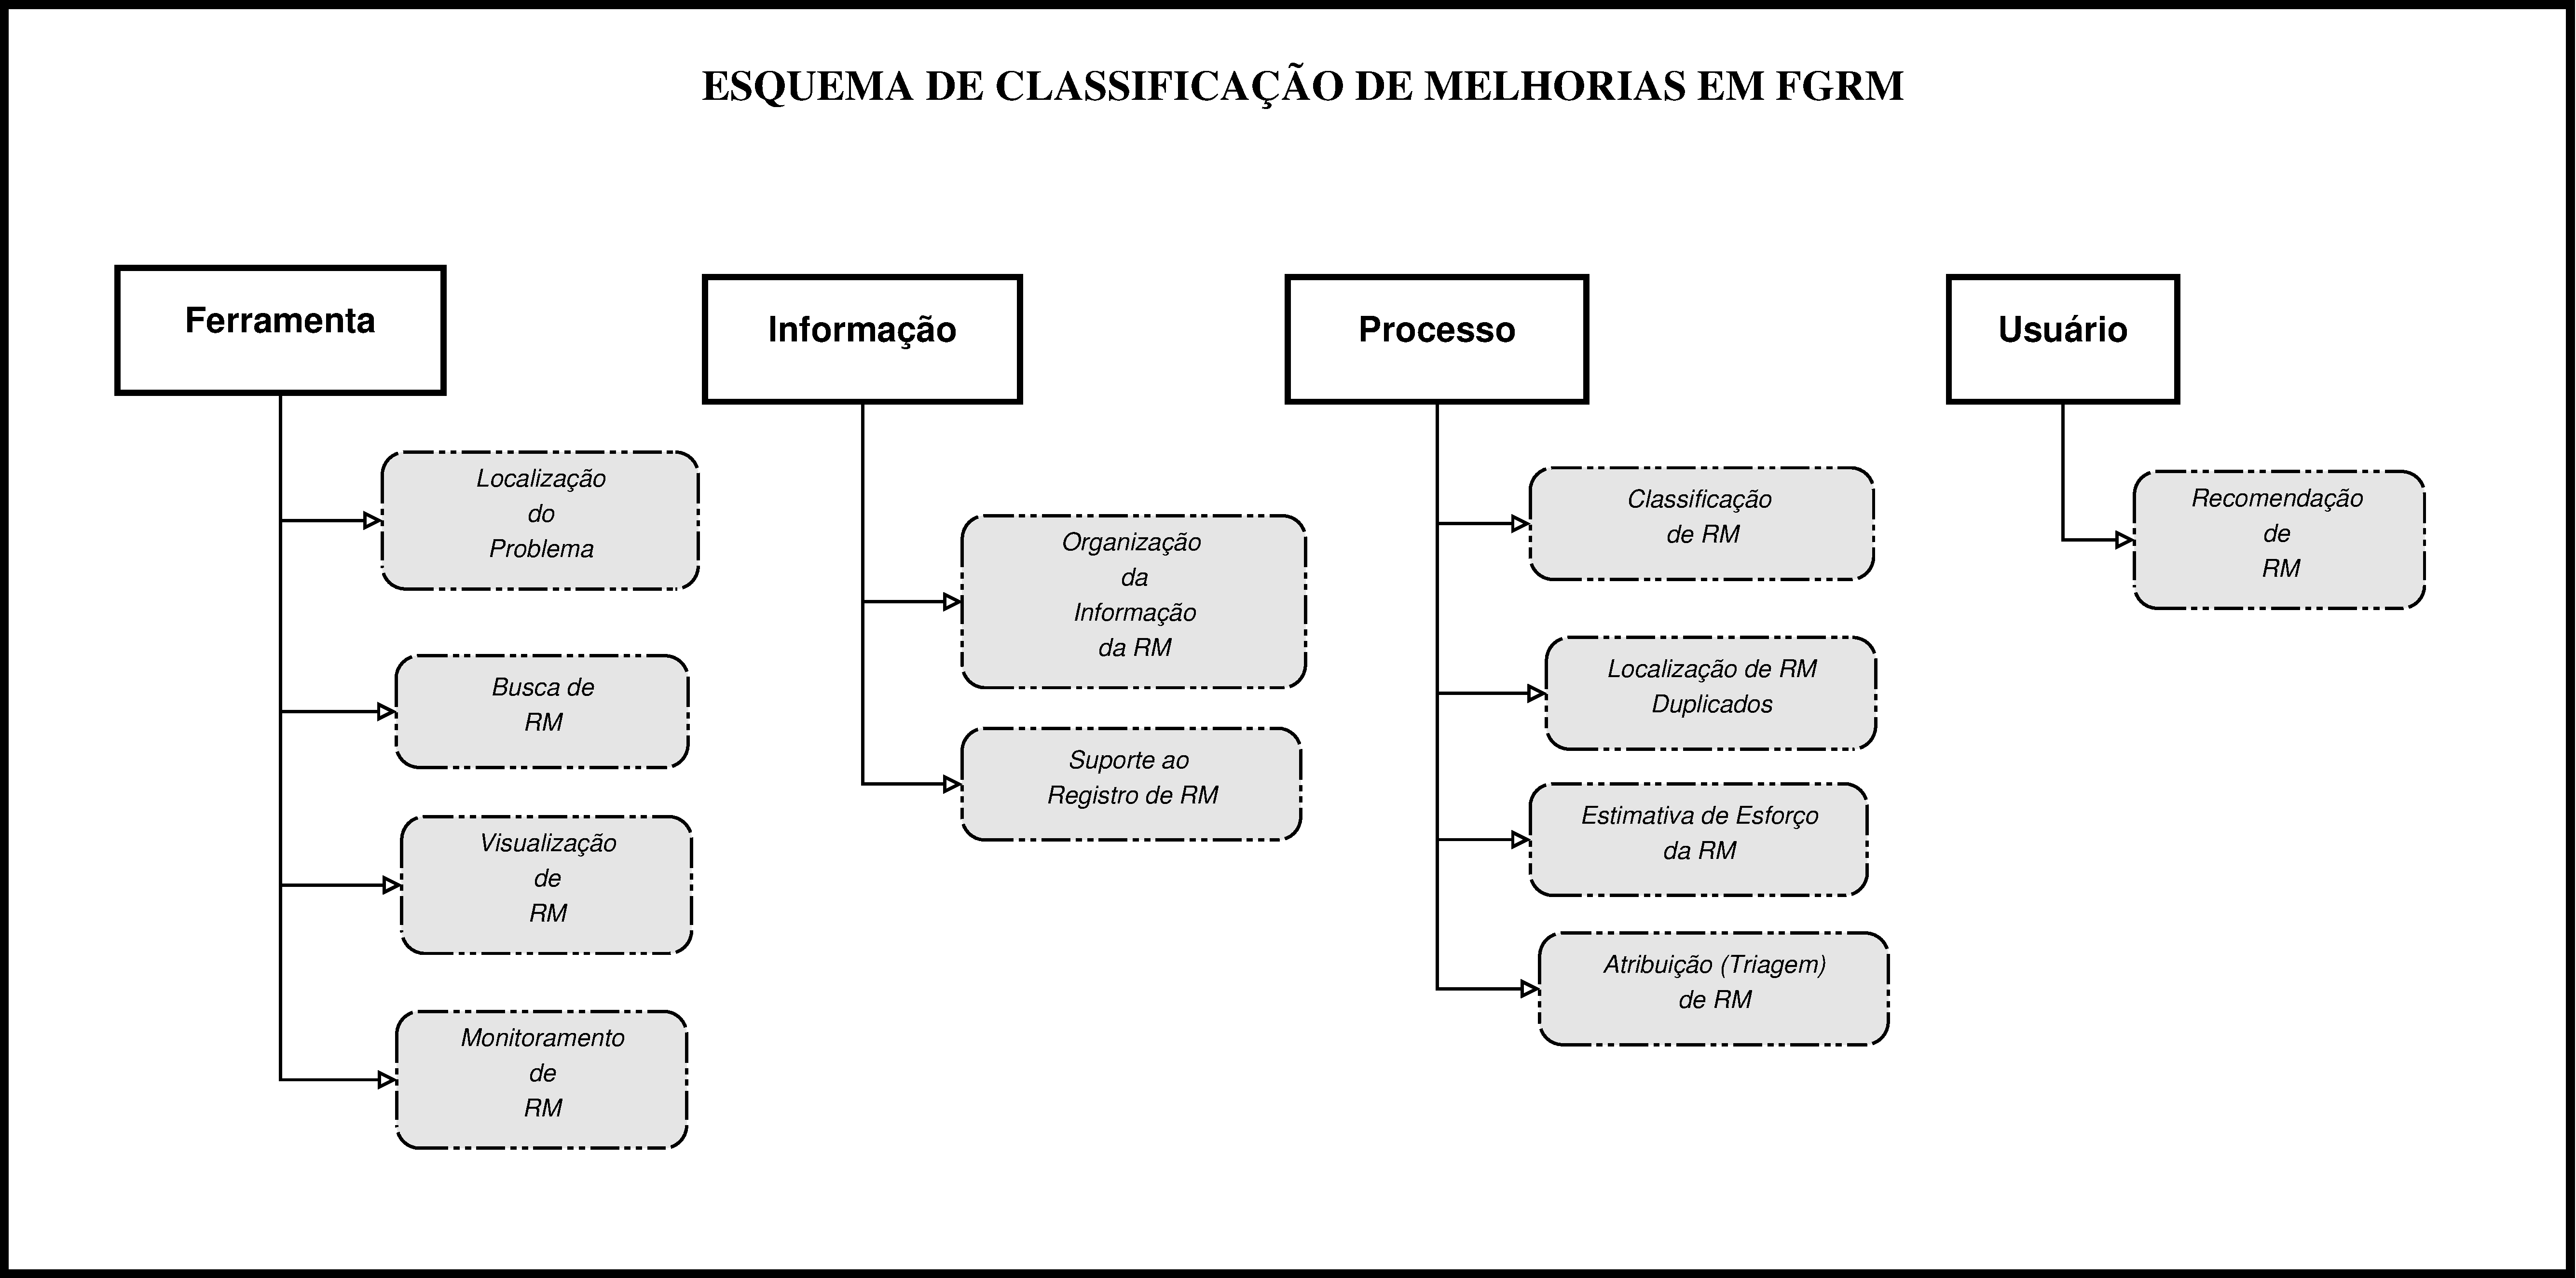
\includegraphics[width=.9\paperwidth]{./chapter-mapeamento-sistematico/img/diagrama-esquema-dimensoes-melhorias.pdf}}
\caption{Esquema de classificação das melhorias propostas na literatura. Os
	retângulos representam as dimensões de melhorias e os polígonos de cantos
	arredondados representam as melhorias.}
\label{fig:diagrama-esquema-dimensao-melhorias}
\end{figure}

\begin{figure}[htpb]
	\centering
	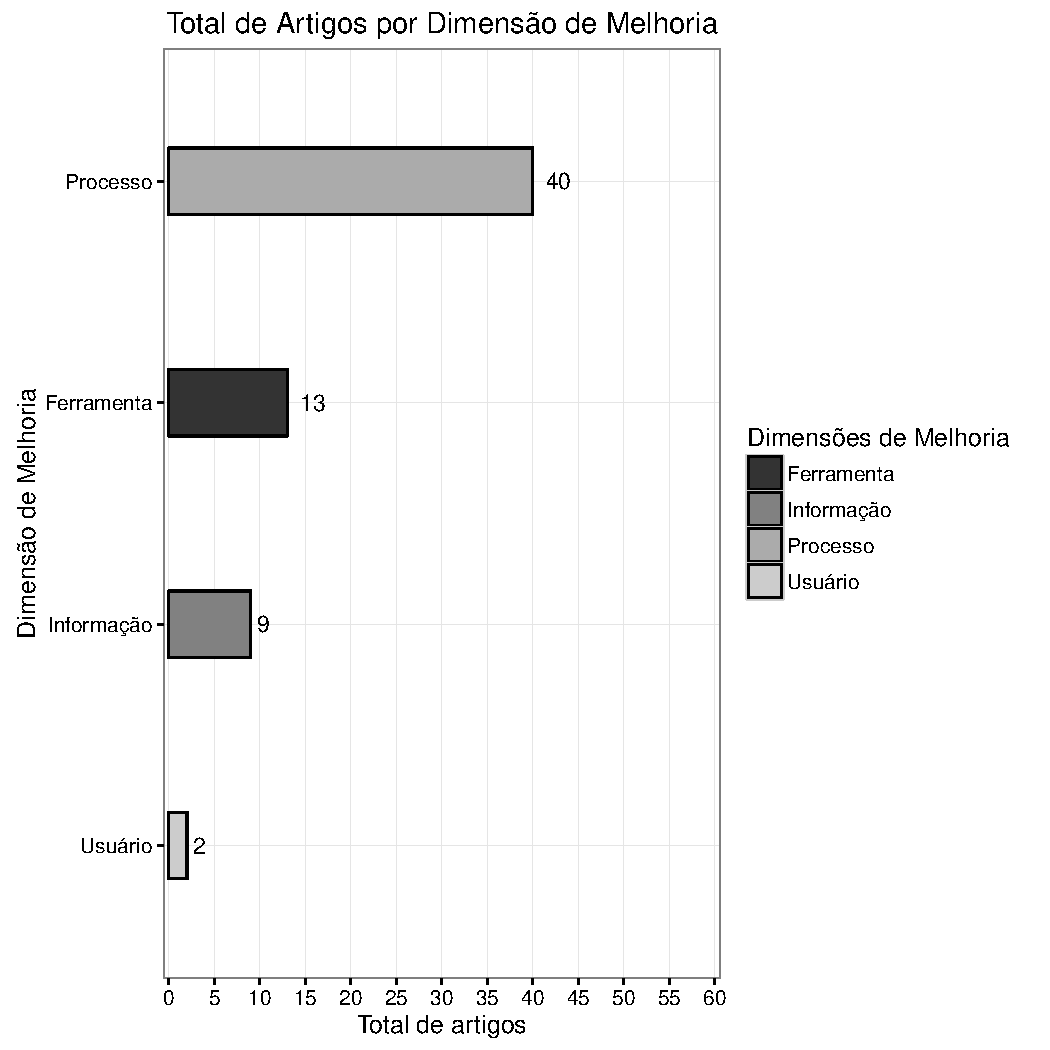
\includegraphics[width=0.9\linewidth]{./chapter-mapeamento-sistematico/img/grafico_dim_melhoria_por_artigo.pdf}
	\caption{Total de artigos por dimensão de melhoria}
\label{fig:grafico_dim_melhoria_por_artigo}
\end{figure}

\begin{figure}[htpb]
	\centering
	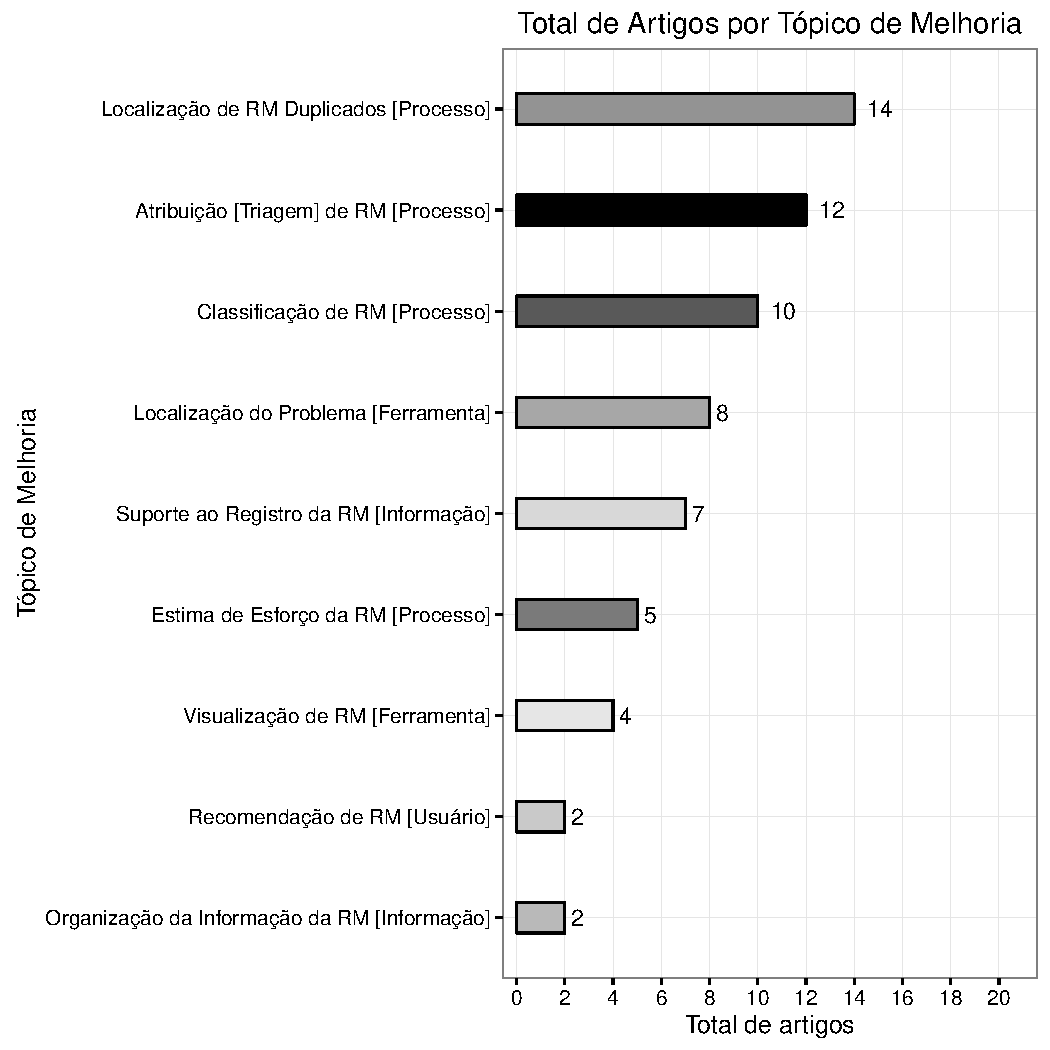
\includegraphics[width=0.8\linewidth]{./chapter-mapeamento-sistematico/img/grafico_topico_por_artigo.pdf}
	\caption{Total de artigos por tópico de melhoria}
\label{fig:grafico_topico_por_artigo}
\end{figure}

\subsubsection{Melhorias Propostas na Dimensão Ferramenta}
\label{ssub:melhorias_dim_ferramenta}

Este ramo do esquema de classificação de classificação proposto foi criada para
agrupar os estudos que discutem melhorias na dimensão Ferramenta. Conforme
anteriormente exposto, esta classe acomoda estudos em tópicos como Localização
	do Problema e Visualização de RM's.
\paragraph{Localização do Problema}
Os estudos incluídos neste tópico de classificação estão devotados ao problema
de localizar a origem de um problema de software com base dos dados da RM\@.
Trata-se do processo de estatisticamente localizar um bug utilizando os dado das
RM's em conjunto com o código fonte~\cite{Hovemeyer:2004:FBE:1052883.1052895}.

A tarefa de encontrar a origem de um falha de software é complexa de consome
muito tempo. Em estudo Lucia e outros relataram que entre 84 a 93\% dos
problemas em software afetam apenas 1~-~2 arquivos de
código-fonte~\cite{thung2012faults}. Contudo não é fácil identificar esses
poucos arquivos dos milhares de arquivos de código-fonte. Esta situação
realça que localizar a origem de um problema (buggy files) é uma tarefa
árdua~\cite{Thung:2014:BIT:2635868.2661678}.

Neste contexto, pesquisadores vem propondo abordagens baseadas em
Recuperação da Informação para localizar falhas com base no que está descritos
nos relatos de bugs. Nessas abordagens existe a tentativa de encontrar entre
o código fonte do sistema um subconjunto de arquivos de fonte que
estão diretamente relacionados à solução do problema
reportado~\cite{Wong:2014:BBF:2705615.2706096}.

Com objetivo de melhorar a eficiência da Localização do Problema diversas
informações contidas nas RM's estão sendo utilizadas. As diversas abordagens
propostas utilizam informações como pilha-erros
(stack-trace)~\cite{Wong:2014:BBF:2705615.2706096}, descrição e campos
estruturados das RM's~\cite{Thung:2014:BIT:2635868.2661678}, o históricos de
versões~\cite{Bangcharoensap:2012:LSC:2419061.2419428,corley2011recovering,Romo:2015:TAT:2745802.2745833}.

Alguns dos estudos propostos foram incluídos em ferramentas largamente
utilizadas no mercado utilizando as propriedades de extensão do
software~\cite{Thung:2014:BIT:2635868.2661678,corley2011recovering}. Os autores
argumentam que pelo fato de nenhuma das técnicas propostas na literatura
estarem integradas às FGRM exite uma dificuldade de adoção da prática da
localização automática de problemas pelos desenvolvedores. Neste sentido, eles
argumentam sobre a necessidade da melhoria das funcionalidades das FGRM em
especial com melhoria ou inclusão de funcionalidades nas FGRM's utilizando o que
vem sendo proposto na literatura.

\paragraph{Visualização de RM}
Os estudos classificados neste tópicos propõe melhorar a visualização das
informações contidas em uma RM\@. A tomada de decisão deve estar subsidiada por
informações corretas. Este fato não é diferente na manutenção e desenvolvimento
de software. Contudo, uma fonte de informação recebeu menos atenção do que o
código fonte: os bugs no sistema. Pouco se sabe sobre o comportamento evolutivo,
o tempo de vida, distribuição e estabilidade dos problemas reportados nas
FGRM~\cite{hora2012bug}. Este problema é reforçado pela forma como as FGRM's
armazenam os dados das RM's. Em geral, esses exibem informações sobre as RM's de
forma textual, o que não é apenas complicado para para navegar, mas também
dificulta a compreensão das intrincadas peças de informação que giram em torno
dos problemas de software~\cite{dal2014bug}.

Com o objetivos de apresentar novas forma de visualizar os dados de uma RM novos
conceitos estão sendo propostos. No estudo de Hora e outros~\cite{hora2012bug} é
apresentado o conceito de Mapa de Bugs (Bugs Maps) que é a ligação de uma RM com
diversos outros artefatos de software como por exemplo o histórico de versões.
No estudo de Lanza e  Dal Sasso~\cite{dal2014bug} o conceito de hiperligação
entre documentos é utilizado para permitir a navegação entre os diversões
artefatos que estão relacionados a um RM\@.

Por outro lado, verificamos o artigo proposto por Takama e
Kurosawa~\cite{takama2013application} onde a aplicação de tecnologias de
visualização de informação foi empregada para o monitoramento das informações
contidas nas RM's. A atualização das informações de uma RM quando gerenciada por
uma FGRM são estruturadas como um fluxo de texto. Contudo, é difícil para as
partes interessadas monitorar uma RM o tempo todo. Neste contexto, a solução
proposta pelo autores visa suportar o monitoramento das RM apresentando ao
usuário mediante animações as atualizações ocorridas em determinada RM\@.

Por conta da natureza das melhorias propostas neste tópico de pesquisa,
verificamos que diversos estudos foram prototipados em ferramentas. Desta forma,
é possível avaliar as propostas através das ferramentas como o
bugMaps~\cite{hora2012bug}, In* Bug~\cite{dal2014bug}.

\subsubsection{Melhorias Propostas na Dimensão Informação}
\label{ssub:melhorias_dim_informacao}

Neste ramo do esquema de classificação foram acomodados os estudos que se propõe
em melhorar a informação que as partes interessadas registram em uma RM\@. Ela é
composta de dois principais tópicos: no primeiro temos o conjunto de
funcionalidades que dão suporte ao registro de uma RM antes que ela seja
armazenada na base de dados de uma FGRM\@; o segundo tópico se dedica aos artigos
que visam organizar a informação já registrada em uma RM, de modo a facilitar o
entendimento por parte dos desenvolvedores e demais profissionais envolvidos na
manutenção de software.

\paragraph{Suporte ao Registro da RM}

Durante o processo de correção de um problema de software verifica-se que a
reprodução manual dos bugs é demorada e tediosa. Os mantenedores de software
rotineiramente tentam reproduzir problemas não confirmados usando as informações
contidas nas RM's que muitas vezes estão
incompletos~\cite{White:2015:GRR:2820282.2820291}. Para complementar os dados
necessários à resolução do problema o desenvolvedor deve solicitar ao
responsável pelo relato da RM as informações necessárias. Os relatos
contidos nas RM's podem conter informações valiosas que podem ser
utilizadas para melhorar a qualidade da informação contidas em novos relatórios
de problemas de software. Esta melhoria da qualidade pode implicar na redução do
custo do processo de garantia de qualidade bem como aumentar a
confiabilidade a confiabilidade do software com a redução gradativa de
bugs~\cite{Tu:2014:MQI:2677832.2677844}.

A pesquisa visando a melhoria da qualidade da informação fornecida nas RM's
começa com estudos visando mensurar de alguma forma os relatos realizadas pelos
usuários. A determinação do que seria um bom relato de um problema de software
foi obtido mediante uma pesquisa (survey) com profissionais devotadas à
manutenção de software~\cite{Bettenburg2008a}. Em outro estudo os autores propõe
as métricas que posteriormente serão utilizadas para avaliar o relato que compõe
a RM~\cite{Tu:2014:MQI:2677832.2677844}.

Um segundo nicho de estudos  nesta área está relacionado ao suporte na
reprodução do erro do software. Estes estudos incluem tanto em registrar o
conjunto de ações que resultaram no erro~\cite{White:2015:GRR:2820282.2820291},
quanto em autocompletar as informações que compõe o relato do
problema~\cite{moran2015auto}. Um ponto em comum deste dois estudos é que eles
foram desenvolvido para o ambiente de desenvolvimento móvel, especial para o
sistema Android~\footnote{\url{https://www.android.com/}}. Uma possível
justificativa para este foco em aplicações móveis pode estar relacionado à
inerente dificuldade em registrar um problema de software naquele ambiente de
software. Neste sentido, a fim de ajudar aos mantenedores a obter relatos de
maior qualidade a melhoria da usabilidade na forma de reportar os defeitos é
importante.

Muitos dos estudos realizados resultaram em ferramentas com a finalidade de
realizar uma prova de conceito no tocante a dar suporte ao usuário em fornecer
um relato de boa qualidade~\cite{Tu:2014:MQI:2677832.2677844, Bettenburg2008a,
	Wu2011a,White:2015:GRR:2820282.2820291,moran2015auto}. Conforme
anteriormente exposto, o desenvolvimento deste protótipos é importante para
fomentar a pesquisa sobre a melhorias das FGRM\@.

\paragraph{Organização da Informação da RM}

	Em alguns casos não é possível aumentar a qualidade da informação fornecida em
um relato de uma RM antes que ela seja armazenada em seu respectivo repositório.
Nestas situações uma abordagem adotada é organizar de uma maneira previamente
definidas as informações contidas em uma RM\@.

Durante o processo de análise de uma RM, em especial para aquelas de caráter
corretiva, existe a tendência dos desenvolvedores em procuram por problemas
semelhantes que foram resolvidos no passado. No entanto, em diversas situações o
desenvolvedor ainda precisa examinar manualmente o conteúdo dos bugs
recomendados que podem variar em tamanho e complexidade~\cite{mani2012ausum}.
Neste contexto, o resumo (sumarização) automático de RM's que tenham relação com
problema em análise é uma maneira de reduzir a quantidade de dados que um
desenvolvedor pode precisa analisar. A ferramenta denominada
AUSUM~\cite{mani2012ausum} propõe uma abordagem, utilizando técnicas não
supervisionadas de IR, de criar este resumo automático de um conjunto de relato
de problemas.

\subsubsection{Melhorias Propostas na Dimensão Processo}
\label{ssub:melhorias_dim_processo}

\paragraph{Localização de RM Duplicadas}
O processo de localização de RM's Duplicadas consiste em avaliar se determinado
relato já foi realizado em algum outro momento. Quando uma RM duplicada é
identificada ele deve ser vinculada a outra que na literatura da área é
denominada como RM Mestre. Geralmente a Mestre é aquela que foi incluída no
repositório de erros em data anterior. Alguns estudos revelam que entre 10\% e
30\% das RM's podem ser classificadas com duplicadas, o que causa um substancial
impacto nas atividades de manutenção de
software~\cite{anvik2005coping,cavalcanti2013bug,Runeson:2007:DDD:1248820.1248882}.
Por conta do grande número de RM's duplicadas se faz necessário designar pessoas
para manualmente analisar as Requisições de Mudanças que chegam com objetivo de
evitar que as duplicatas cheguem as desenvolvedores~\cite{anvik2005coping}.

O processo de identificação de RM's duplicadas requer um prévio conhecimento do
conjunto de relatos existentes previamente no projeto ou mediante a busca manual
em toda base de dados da FGRM~\cite{banerjee2012automated,
	Lerch:2013:FDY:2495256.2495763,hindle2016contextual}. Ambas as estratégias
consomem tempo e não garantem que falso positivos possam
ocorrer~\cite{kaushik2012comparative}. Os falso positivos podem ainda acarretar
em caso de relevantes problemas do software relatados pelo usuários serem
desconsideradas.

A abordagem adotada da literatura para tratar o problema das RM's duplicadas
podem ser divididas em dois tipos\cite{kaushik2012comparative,
	tian2012improved}: \textit{(i)} remoção de duplicatas, \textit{ii}
identificação de duplicatas, que agrupa grande parte da pesquisa no
assunto~\cite{cavalcanti2014challenges}. No primeiro tipo, o objetivo é evitar
que RM duplicadas entrem na base de dados de uma FGRM e desta forma evitar o
esforço e o tempo extra necessário para identificá-la posteriormente.

Por outro lado, o segundo tipo não se importa se duplicados entram na base de
dado de RM's. Não obstante, o objetivo é sugerir uma lista de possíveis
duplicatas durante o processo de registro de uma nova RM e possivelmente
agrupá-los. Um ponto importante para se ressaltar é que este segundo tipo se
baseia na premissa que registrar um mesmo problema por mais de uma vez nem
sempre é problemático tendo em vista que pode fornecer informações adicionais
que podem ser úteis~\cite{bettenburg2008duplicate}. No entanto, alguns estudos
compensam o custo de sua recuperação e permanência na base de dados de
RM's~\cite{davidson2011coping}. Neste sentido, é importante que novas
abordagens tentem equilibrar este dois tipos de abordagem de movo a evitar o
tempo extra para análise de uma RM bem como apoiar os desenvolvedores com
informações adicionais~\cite{Lerch:2013:FDY:2495256.2495763,Thung2014}.

\paragraph{Atribuição (Triagem) de RM}
O processo de atribuição de RM, também conhecido como \textit{triagem}, possui
como principal objetivo encontrar o desenvolvedor mais capacitado para manipular
uma dada RM~\cite{cavalcanti2014challenges}. Existe a premissa que a escolha do
desenvolvedor apropriado é crucial para obter um menor tempo para resolução de
determinada RM~\cite{di2002approach}. Estudos também discutem que o processo de
atribuição deve considerar fatores tais como a carga de trabalho do
desenvolvedor a prioridade da RM~\cite{aljarah2011selecting}.

\paragraph{Classificação da RM}
Independentemente do tipo e tamanho de um projeto é sempre importante determinar
qual tipo manutenção deverá ser realizada tomando como base o relato de uma RM\@.
Este processo consiste de forma resumida em classificar uma requisição com base
em algum esquema de classificação previamente definido. Este esquema pode ser
classificar em \textit{corretiva, perfectiva, preventiva ou
	adaptativa}~\cite{4425813} ou mesmo como \textit{resolver um problema de
	software} ou \textit{implementar uma melhoria.}
A diversa de categorias em determinado esquema de classificação  pode tornar
complexo a tarefa, tendo em vista que em muitos casos não é fácil determinar os
limites entre os tipos~\cite{antoniol2008bug}. Por exemplo, a uma classificação
incorreta de um defeito como melhoria pode acarretar em atrasos no projeto ou
mesmo fazendo que uma RM receba menos atenção do que ela
mereça~\cite{cavalcanti2014challenges}.

\paragraph{Estimativa de Esforço da RM}
A gestão do custo e esforço de um projeto de manutenção de software passa pelo
controle do esforço necessário ao cumprimento de suas RM's. Os estudos que medem
o esforço de uma RM utilizam em geral três forma para medir este
esforço~\cite{cavalcanti2014challenges}: determinar o tempo para solucionar
novas RM's; determinar os artefatos que são impactados por determinada RM;
prever o número de novas RM's que poderão fazer parte do projeto.

No primeiro tipo de estudo a preocupação é estimar o tempo necessário para
tratar a mudança solicitada em determinada requisição. Naturalmente, existe uma
 complexidade produzir uma estimativa precisa por conta das
diferentes atividades envolvidas em conjunto aos diferente níveis de capacitação
que o responsável pela execução das tarefas pode ter~\cite{xia2015automatic}.
Apesar da inerente imprecisão deste tipo de trabalho é importante salientar que
estimar o tempo de solução de uma RM é importante para o gerenciamento do
projeto porque ajudar alocar recurso de forma mais
eficiente~\cite{Bhattacharya:2011:BTP:1985441.1985472} e melhorar a previsão do
custo necessário para o lançamento de futuras versões do
sistema~\cite{Vijayakumar2014}.

No segundo grupo temos os artigos que tentam identificar previamente o conjunto
de artefatos que serão impactados pela tarefa de manutenção~\cite{Nagwani2010}.
\todo[inline]{Incluir citação para o artigo Impact analalysis by mining .. e
	Identifing the start impact set of a }. A literatura sobre análise de
impacto é bastante abrangente e pode envolver o estudos de artefatos tais como
documentos de requisitos e arquiteturais dos software, código fonte, registros
(logs ) de teste e assim por diante~\cite{cavalcanti2014challenges}. Neste
sentido,estamos focados em estudos onde a RM são o ponto de partida para a
análise de impacto.

O último grupo de trabalho se dedica em prever o número de RM que possivelmente
serão relatadas em futuras versões do sistema. De forma similar ao primeiro
grupo este tipo de estudo visa contribuir com o planejamento das atividades de
manutenção e evolução. A predição do que será relatado incluí tanto novas
requisições de problemas que não existiam em versões anteriores, por exemplo,
\todo[inline]{Inserir citação de Software defect association mining and
	defects  e  Minig software code repositories and bug database...}, bem
como aqueles que serão reabertos, ou seja, problemas que não foram solucionados
anteriormente mesmo as suas RM's dizendo o contrário~\cite{xia2015automatic}

\subsubsection{Melhorias Propostas na Dimensão Usuário}
\label{ssub:melhorias_dim_usuario}

\paragraph{Recomendação de RM}
Os estudos contidos neste tópico possuem foco em dar suporte à novos
desenvolvedores na redução da curva de aprendizagem quando eles pretendem
ingressar em um um novo projeto. Por exemplo, quando um novo desenvolvedor entra
na equipe seria interessante que ele resolvesse as RM's que tivessem um menor
nível de dificuldade. Posteriormente, quando o desenvolvedor ganhasse
experiência, poderia aumentar o grau de dificuldade relacionado à RM que ele
deve tratar. Este tipo de processo ocorre com certa frequência em projetos de
código aberto, onde a contribuição de desenvolvedores fora do projeto é
fundamental.No entanto, encontrar um bug apropriado e uma correção apropriada
para esse bug requer uma boa compreensão do projeto, que não é
trivial~\cite{Wang2011bug}.

Em algum projetos, um membro experiente da equipe, geralmente ensina os
recém-chegados o que eles precisam para fazer completar suas tarefas necessárias
à conclusão de uma RM. Todavia, alocar um membro experiente de uma equipe para
ensinar um recém-chegado durante um longo tempo nem sempre é possível ou
desejável, porque o mentor poderia ser mais útil fazendo tarefas mais
importantes~\cite{malheiros2012source}.

Para facilitar a inclusão de novos desenvolvedores alguns estudos vêm se
dedicando em desenvolver sistemas de recomendação de
RM's~\cite{malheiros2012source, Wang2011bug}. Estes sistemas de recomendação
podem ajudar o recém-chegado a solucionar uma RM mediante a apresentação de
outras de código fonte potencialmente relevante que o ajudará na solução da RM
do qual ficou responsável~\cite{malheiros2012source}.

O segundo tipo de abordagem pode ser vista como ambiente de exploração do
repositório de RM's.  Este tipo de funcionalidade permite que permitir que novos
desenvolvedores pesquisem descrições das requisições que possam ser do seu
interesso bem como dos artefatos relacionados àquela RM (por exemplo, arquivos
relacionados, desenvolvedores contribuintes, registros de
comunicação)~\cite{Wang2011bug}.

Com base nos estudos que compõe esta categoria, verificamos que modelos de IR
vêm sendo utilizados para possibilitar a recomendação de RM. Neste contexto,
técnicas bem conhecidas na literatura tais como VSM~\cite{Wang2011bug} e o
modelo estatístico PPM~\cite{malheiros2012source}.

\subsection{Classificação por Melhorias com Suporte à Papéis da Manutenção de
	Software}
\label{sub:extensões_com_suporte_a_papeis}
\todo[inline]{Verificar os artigos com N/A e não especificado}
Nesta seção apresentamos a classificações dos estudos pelo tipo de papel na
manutenção de software ao qual a funcionalidade visa dar suporte. Conforme
exposto anteriormente a definição dos compõem o processo de manter de software
foi desenvolvido conforme os trabalhos realizados por Polo e
outros~\cite{Polo1999} e Ihara e outros~\cite{Ihara:2009:AMI:1595808.1595833}\@.
Com esta modificações é possível acoplar os papéis utilizados neste estudo tanto
aos processo adotados na indústria e em projetos de código aberto. A
Figura~\ref{fig:graf_papel_por_artigo} exibe o total de artigos em comparação
com o papel ao qual funcionalidade proposta visa dar suporte. Como pode ser
observado verificamos um maior número de estudos para os papéis de Agendador e
Desenvolvedor. Na Figura~\cite{fig:grafico_topico_por_artigo} verificamos uma
prevalência de estudos com foco na dimensão Processo, em especial nos tópicos
"Localização de RM Duplicados" e "Atribuição [Triagem] de RM", o que  é natural
tendo em vista que há um mapeamento o papel desempenhado na manutenção com as
atividades desempenhada por aquele papel. Neste sentido, não é de se estranhar a
prevalência de estudos para aqueles funções vinculada ao processo de manutenção
de software.

\begin{figure}[htpb]
	\centering
	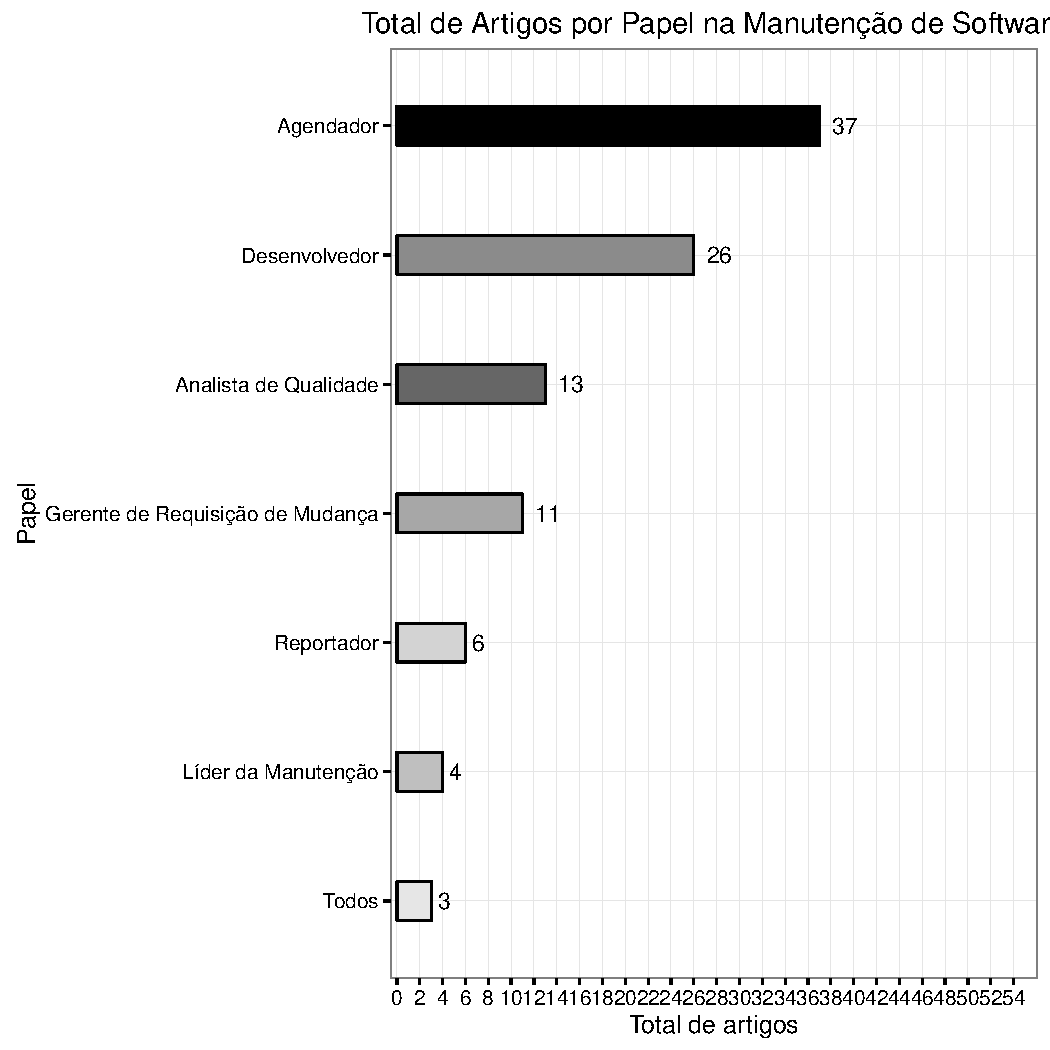
\includegraphics[width=0.8\linewidth]{chapter-mapeamento-sistematico/img/grafico_papel_por_artigo.pdf}
	\caption{Total de artigos por papel na manutenção de software}
	\label{fig:graf_papel_por_artigo}
\end{figure}

\paragraph{Agendador}
O estudos classificados neste tópico visam dar suporte as atividades de
Agendador. Esta função têm como principal objetivo atribuição das RM’s
para o desenvolver mais apto~\cite{banitaan2013decoba}. O processo de atribuição
de RM's deve ser realizado em acordo com a carga de trabalho do desenvolvedor e
com a prioridade que foi atribuída à RM~\cite{chawla2015automated}. 

Neste contexto, os estudo têm focado em apresentar soluções de atribuição
automática~\cite{banitaan2013decoba, shokripour2012automatic,
	somasundaram2012automatici,Naguib2013, Zhang2014, Zanetti2013}; classificação
automatizada~\cite{gegick2010identifying,liu2014faceted, behl2014bug,
	chawla2015automated,tian2015automated}; visualização da
fila de RM's~\cite{izquierdo2015gila}; clusterização das
requisições~\cite{liu2014faceted}; determinação do tempo necessário à conclusão
da RM (time do fix)~\cite{hosseini2012market,
	Bhattacharya:2011:BTP:1985441.1985472}; sumarização das informações
contidas na RM~\cite{mani2012ausum}; determinação de RM'S
duplicadas~\cite{Sun2011, Wu2011a}.

Apesar da lista de artigos apresentada em cada tópico não ser exaustiva, os
resultados demonstram um foco maior no suporte à atribuição e categorização das
RM's apresentado soluções automatizadas para estas atividades. Existe
possivelmente uma crença melhorar a produtividade do processo de manutenção de
software reduzindo o esforço de encontrar o desenvolvedor mais apto.

\paragraph{Desenvolvedor}
Ao Desenvolvedor cabe aplicar as ações que irão produzir o resultado
solicitado/esperado na RM. Os estudos nesta categoria deveriam suportar
atividades tais como codificação, depuração e testes. 

No suporte ao desenvolvedor verificamos estudos que propõe à atribuição de RM's
ao conjunto de desenvolvedor, em contrapartida da tradicional atribuição ao
único programador~\cite{banitaan2013decoba}, visando da minimizar o problemas
decorrentes à propriedade de código e propiciar um maior nivelamento de
informações entre os membros da equipe. Não obstante, o maior grupo de estudos
nesta categoria estão relacionados na ajuda ao desenvolvedor de vincular um
determinado problema do software à sua efetiva origem, ou seja, ao código
fonte~\cite{corley2011recovering,Wong:2014:BBF:2705615.2706096,
	Thung:2014:BIT:2635868.2661678,Nguyen:2012:MAR:2393596.2393671,thung2013automatic,
	Romo:2015:TAT:2745802.2745833}. Neste mesma categoria verificamos estudos
que dão suporte ao desenvolvedor em classificar à RM que lhe foi atribuída, em
especial aquelas que estão relacionadas às questões de segurança do
sistema~\cite{gegick2010identifying} ou aquelas RM's que possam impedir a
resolução de outras
(blocking-bugs)~\cite{ValdiviaGarcia:2014:CPB:2597073.2597099}

\paragraph{Analista de Qualidade}
Cabe ao Analista de qualidade avaliar se uma RM foi solucionada por um
Desenvolvedor afim de verificar se a RM foi corretamente resolvida. Neste
sentido, melhorias em FGRM's que visam facilitar as atividades deste papel podem
estar relacionadas ao processo de teste de software.

De maneira similar ao que ocorre na categoria de Desenvolvedor verificamos uma
prevalência dos estudos visam determinar uma ligação entre um problema de
software o código
fonte~\cite{corley2011recovering,Wong:2014:BBF:2705615.2706096,
	Thung:2014:BIT:2635868.2661678,Nguyen:2012:MAR:2393596.2393671,thung2013automatic,
	Romo:2015:TAT:2745802.2745833}. Verificamos ainda estudos que tentam
predizer a probabilidade que determinada RM será
reaberta~\cite{xia2015automatic}, o que pode ajudar ao
Analista de Qualidade na priorização das requisições com alta possibilidade de
reabertura

\paragraph{Gerente de Requisição de	Mudança}
O papel que representa esta categoria está vinculado à gestão do processo de
manutenção de software, em especial por decidir se uma Requisição de Mudança
será aceita ou rejeitada. Neste contexto, melhorias relacionadas à classificação
quanto ao nível de segurança~\cite{gegick2010identifying, zhang2011bug,
	ValdiviaGarcia:2014:CPB:2597073.2597099}, identificação de
duplicados~\cite{hindle2016contextual, sun2010discriminative,
	alipour2013contextual, banerjee2012automated}. 

O estudos que fazem parte desta categoria destacam que um considerável
conhecimento sobre o projeto é necessário bem como  a capacidade de negociação
com os desenvolvedores e demais partes interessadas são importantes para
desempenho de papel. Todavia, tendo em vista o esforço e tempo gasto por esta
tarefa, especialmente quando realizada manualmente, seria importante que as FGRM
automatizasse algumas destas atividades.

\paragraph{Reportador}
Conforme discutido anteriormente os dados contidos nas RM'S são fundamentais em
em diversas abordagens de melhorias da funcionalidades das FGRM. Esta relevância
ainda é maior nos estudos que fazem uso de técnicas de Recuperação da
Informação. Neste sentido é importante que as FGRM deem suporte ao Reportador
que, na maioria, é primeiro a registrar as informações que serão necessárias à
solução da RM. 

Muitos dos estudos que fazem parte desta categoria  partem da premissa que
melhorar a qualidade dos dados na RM é o ponto de partida para tratar outros
problemas relacionados ao processo de manutenção de
software~\cite{moran2015auto, Moran:2015:EAA:2786805.2807557, Bettenburg2008a}.
Neste sentido verificamos estudos para autocompletar as informações fornecidas
pelo Reportador~\cite{moran2015auto}, suporte a reprodução do
problema~\cite{Moran:2015:EAA:2786805.2807557}; análise da qualidade da
informação fornecida~\cite{Bettenburg2008a, Tu:2014:MQI:2677832.2677844}. Esta
categoria também contempla um estudo que visa detectar que determinada RM já foi
registrada durante o processo de escrita da mesma~\cite{Thung2014}.
\paragraph{Líder da Manutenção}
De forma similar ao Gerente de Requisição de Mudança as melhorias de
funcionalidades proposta nesta categoria estão vinculadas à gestão de manter
software. Conforme o esquema de  classificação de papeis utilizado neste estudo,
o Líder da Manutenção têm por responsabilidade definir os padrões e
procedimentos que compõe o processo de manutenção que será utilizado. Para
ajudar nesta tarefa alguns estudo  vêm propondo melhorar a alocação de Tarefas
do processo de resolução das Requisições de Mudanças~\cite{netto2010automated}.
Outros estudos visam mensurar o esforço necessário para solucionar determinada
RM~\cite{Vijayakumar2014, Nagwani2010}, o que podem ajudar ao Líder no
planejamento de liberações de novas versões do sistema que está sendo mantido. 

\paragraph{Todos}
Esta categoria abarca os estudos para o qual a melhoria proposta possui impacto
positivo para todos os papéis envolvidos na manutenção de software. A definição
que o foco da melhoria é geral decorre do que foi dito como objetivos dos
autores dos estudos que fazem parte desta categoria ou ainda por não ser
possível determinar uma atividade específica sendo beneficiada.

Conforme pode ser observado, os estudos estão relacionados principalmente com a
melhoria da  visualização das informações contidas nas RM's~\cite{hora2012bug,
	takama2013application, dal2014bug}. As melhorias podem estar vinculadas a
questões de usabilidade das ferramentas, como por exemplo a navegabilidade entre
as RM's~\cite{dal2014bug}. 

\subsection{Ferramentais Estendidas}
\label{sub:ferrramentas_extendidas}

Conforme verificamos nas seções anteriores diversos estudos vêm sendo propostos
na literatura com o objetivo de melhorias atividades relacionadas à manutenção
de software. Não obstante, os nosso resultados demostraram, tomando como base os
estudos que fazem parte deste mapeamento, que grande parte das melhorias
propostas não foram implementadas nas FGRM de modo a ser utilizadas ou avaliadas
pelo profissionais envolvidas em manutenção de software. 

A Figura~\ref{fig:grafico_virou_extensao} apresenta a quantidade de estudos que
efetivamente foram transformadas em extensões de funcionalidades de uma FGRM.
Do total de 64 estudos que foram utilizados neste mapeamento apenas fazem parte
das funcionalidade de uma FGRM. 
\todo[inline] {reavaliar a quantidade de estudos}. 

\begin{figure}[htpb]
	\centering
	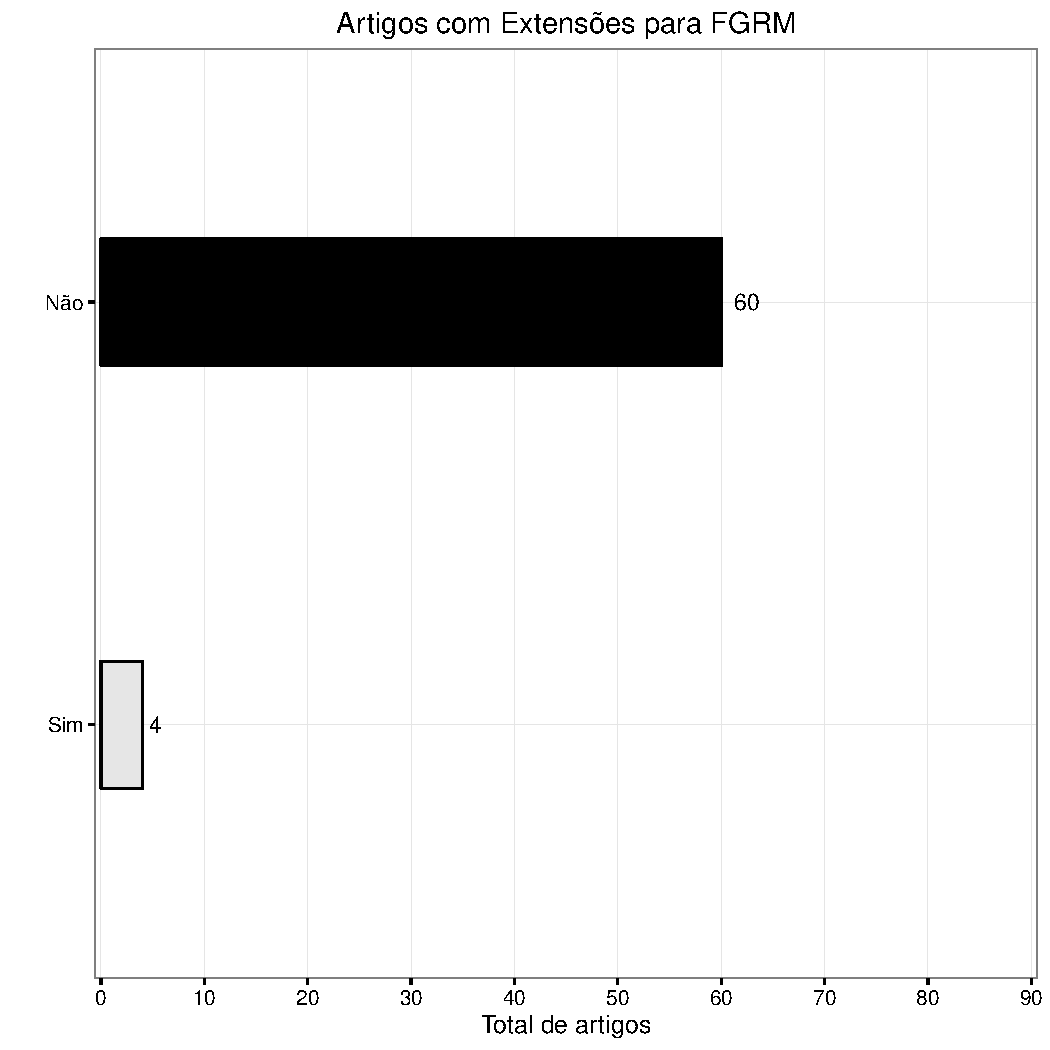
\includegraphics[width=0.8\linewidth]{chapter-mapeamento-sistematico/img/grafico_virou_extensao.pdf}
	\caption{Total de estudos que são extensões para FGRM}
	\label{fig:grafico_virou_extensao}
\end{figure}

Cabe ressaltar que no escopo de determinado estudo pode não esta prevista a
efetiva transformação da melhoria proposta de modo a ser utilizada efetivamente
pelo seu público-alvo, como por exemplo, a criação ou melhoria de uma
funcionalidade de determinada FGRM. Ademais, não está no escopo deste estudo
avaliar ou discutir a facilidade que as FGRM possuem para criar novas
funcionalidades ou melhorias as já existentes. Contudo, o nosso entendimento é
que como um maior número de melhorias proposta na literatura sendo utilizadas
pelos profissionais envolvidos em manutenção de software poderia melhorar a
qualidade das soluções propostas mediante a redução da diferença entre o
estado-da-prática com o estado-da-arte. 

\section{Discussão}
\label{sec:discussao}


\section{Limitações e Ameaças à Validade}
Questões de pesquisa: É possível que as perguntas de pesquisa definidas possam
não abranger completamente o campo dos repositórios de RC. No entanto, algumas
discussões com membros do projeto e especialistas em Manutenção de Software
foram realizadas para validar as perguntas. Assim, mesmo que não tenhamos
considerado o melhor conjunto de questões, tentamos abordar as questões mais
frequentes e abertas no campo, tanto do ponto de vista do praticante como do
investigador.

Vieses de publicação: Não é possível garantir que todos os estudos primários
relevantes foram selecionados e alguns estudos relevantes não podem ser
escolhidos durante o processo de busca. Essa ameaça foi atenuada pelas
referências a seguir nos estudos primários, em uma técnica chamada bola de neve
[22]. No entanto, devido ao volume de artigos coletados, acreditamos que a
pesquisa no campo está bem representada. Em outras palavras, os possíveis
documentos em falta não teriam um impacto significativo nos resultados deste
estudo de mapeamento.

Pesquisa realizada: Como as bases de dados digitais não funcionam com regras de
pesquisa compatíveis entre si, todas as sequências de pesquisa foram adaptadas e
calibradas para cada banco de dados digital. No entanto, não conhecemos todas as
regras que as bases de dados digitais utilizam para procurar um documento. Isso
foi atenuado pela

Extração e classificação dos dados: Durante o processo de extração, os estudos
foram classificados com base em nosso julgamento. No entanto, apesar da dupla
verificação, alguns estudos poderiam ter sido classificados incorretamente. Além
disso, às vezes era difícil classificar os estudos, de acordo com áreas de
pesquisa e tópicos, devido à estreiteza entre desafios e oportunidades. Para
mitigar isso, o processo de classificação foi repetido por cada autor deste
estudo e os resultados foram discutidos em conjunto a fim de chegar a um
consenso


\section{Trabalhos Relacionados}
Kagdi et ai. [159] realizou uma revisão da literatura sobre abordagens para
repositórios de software de mineração sobre a evolução e manutenção de software.
O resultado foi uma taxonomia baseada em quatro dimensões: o tipo de repositório
extraído (o que), o propósito (por que), o método proposto (como) e o método de
avaliação (qualidade). No entanto, sua taxonomia não fornece um entendimento
extensivo sobre as investigações em repositórios de RC, principalmente por duas
razões. Em primeiro lugar, embora pesquisassem muito trabalho e fizessem uma
taxonomia consistente, isso foi feito já em 2006 e desde então muitos outros
trabalhos foram publicados, considerando novos tópicos e abordagens. Em segundo
lugar, de acordo com seus critérios de exclusão para estudos, eles estavam muito
preocupados com estudos que abordavam mudanças evolutivas de artefatos de
software investigando múltiplos repositórios de software. Como consequência,
muitos estudos que usaram dados de um repositório único estavam além de seu
escopo, como aqueles que se baseavam apenas em dados de repositórios de CR.

Por outro lado, nosso estudo de mapeamento sistemático reduziu o foco para
investigações sobre CR Repositórios, para que possamos fornecer uma visão
abrangente do estado da arte sobre este tópico. As dimensões propostas por Kagdi
et al. [159] Foram utilizados para orientar a análise dos estudos que
consideramos neste artigo. Além disso, também analisamos algumas ferramentas e
serviços para entender a transferência de tecnologia ao investigar repositórios
de CR. Outra diferença de Kagdi et al. [159] é que sua taxonomia considera as
técnicas e métodos para repositórios de software de mineração como entidades de
primeira classe, enquanto a nossa análise se concentrou nos desafios e
oportunidades relacionados aos repositórios de CR. Assim, passamos dos detalhes
do Como para os detalhes da dimensão Por que resulta em uma taxonomia das áreas
de pesquisa dos repositórios de CR. Além disso, vale a pena mencionar que,
embora mudássemos o foco da taxonomia, não negligenciamos os aspectos técnicos
das abordagens identificadas em cada tópico da taxonomia

\section{Resumo do Capítulo}